\chapter{Λογική Μετάθεση Πλαισίων}
\label{chap5}

\section{Εισαγωγή}
\label{chap5_Intro}

Σύμφωνα με την έως τώρα ανάλυση, εξάγεται το συμπέρασμα πως η μείωση του αριθμού των πλήρως ελαττωματικών συνόλων θα συνέβαλε σημαντικά στη μείωση των επιπτώσεων που προκαλεί η ύπαρξη ελαττωματικών στοιχείων στον Πίνακα Πρόβλεψης Προορισμού Διακλάδωσης. Στο παρόν κεφάλαιο παρουσιάζεται μία νέα αυτοματοποιημένη τεχνική για την λογική μετάθεση των πλαισίων του πίνακα, με ελάχιστο κόστος. Η τεχνική αυτή συνοδεύεται από ένα αλγόριθμο ο οποίος παρουσιάζεται υπό δύο μορφές. Στην πρώτη μορφή του όλα τα βήματα εκτελούνται σειριακά, ενώ στη δεύτερη γίνεται χρήση παραλληλίας για ταχύτερο υπολογισμό.

%----------------------------------------------------------%

\section{Στόχος}
\label{chap5_Target}

Όπως αναφέρθηκε στο Κεφάλαιο \ref{chap2} ο Πίνακας Πρόβλεψης Προορισμού Διακλάδωσης, αποτελούνται από τ πλαίσια ανά σύνολο (Πλαίσιο-0 έως Πλαίσιο-[τ-1]) στα οποία συμπεριλαμβάνονται τα πεδία ετικέτας, διεύθυνσης προορισμού και ορισμένες επιπλέον πληροφορίες. Από την ανάλυση που έγινε στο Κεφάλαιο \ref{chap4} είναι φανερό πως η μείωση της επιβάρυνσης στην απόδοση εξαιτίας των σφαλμάτων στον Πίνακα Πρόβλεψης Προορισμού Διακλάδωσης μπορεί να επιτευχθεί μέσω του περιορισμού των πλήρως ελαττωματικών συνόλων, δηλαδή την καλύτερη κατανομή των ελαττωματικών πλαισίων ανάμεσα στα σύνολα.
\par
Στην ακόλουθη προτεινόμενη τεχνική, για την επίτευξη του στόχου χρησιμοποιείται η γνώση των θέσεων των ελαττωματικών πλαισίων του πίνακα, πληροφορία η οποία βρίσκεται αποθηκευμένη στα ψηφία σφάλματος. Οι τιμές αυτές εξάγονται μέσω της διαδικασίας ανίχνευσης λαθών στα στοιχεία μνήμης, όπως παρουσιάστηκε στο Κεφάλαιο \ref{chap3}, και αποθηκεύονται σε κατάλληλες δομές ώστε με τη μεταβολή της τάσης λειτουργίας να γίνεται και η ενημέρωση των αντίστοιχων ψηφίων σφάλματος. Για την καλύτερη επεξήγηση της τεχνικής ο πίνακας τ-τρόπων συνόλου συσχέτισης διαχωρίζεται σε τ τμήματα πλαισίων (Τμήμα-0 έως Τμήμα-[τ-1]). Έτσι το Τμήμα-0 θα περιέχει τα Πλαίσια-0 όλων των συνόλων, όπως παρουσιάζονται και στο Σχήμα \ref{fig:chap5_btb_init}.

\begin{figure}[t]
    \centering
    \fbox{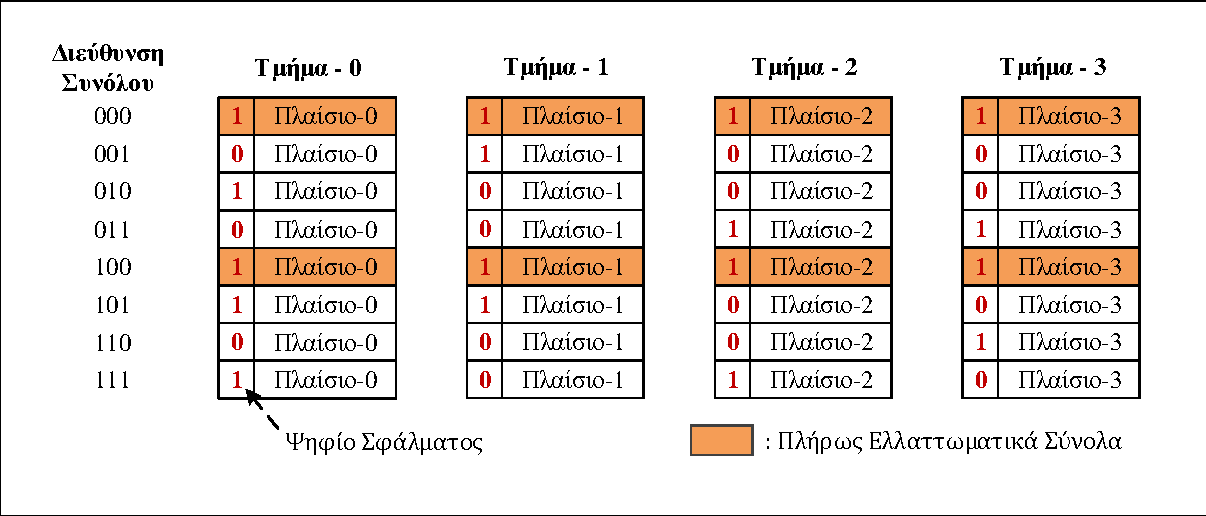
\includegraphics[width=\linewidth, trim=0.8cm 0.9cm 0.7cm 0.7cm, clip=true]{\algorithmsDIR/chap5_example.pdf}}
    \caption{Πλαίσια, σύνολα και τμήματα του Πίνακα Πρόβλεψης Προορισμού Διακλάδωσης}
    \label{fig:chap5_btb_init}
\end{figure}

Με βάση τις θέσεις των ελαττωματικών πλαισίων σε κάθε τμήμα, υπολογίζονται κατάλληλες τιμές οι οποίες αποθηκεύονται σε ένα ξεχωριστό καταχωρητή για κάθε τμήμα, τον αποκαλούμενο ως $``$Καταχωρητή Διαμόρφωσης$"$, ο οποίος χρησιμοποιείται για την τροποποίηση της διεύθυνσης πλαισίου του τμήματος. Η τελική διεύθυνση προσπέλασης (\textit{ΔΠ}) στην κάθε τμήμα παράγεται από τη συνάρτηση \xor μεταξύ του πεδίου διεύθυνσης (\textit{ΠΔ}) της εντολής διακλάδωσης και της τιμής του καταχωρητή διαμόρφωσης του τμήματος (\textit{ΚΔ}):
\begin{equation}
    \textit{ΔΠ(Τμήματος-Χ)} = \textit{ΠΔ} \oplus \textit{ΚΔ(Τμήματος-Χ)}
\end{equation}
\par
Με τον τρόπο αυτό γίνεται ανακατεύθυνση των προσπελάσεων με διαφορετικό τρόπο σε κάθε τμήμα δημιουργώντας έτσι νέα σύνολα πλαισίων τα οποία αποκαλούνται $``$Λογικά Σύνολα$"$. Σκοπός του αλγορίθμου που παρουσιάζεται στο παρόν κεφάλαιο είναι ο υπολογισμός κατάλληλων τιμών για τους Καταχωρητές Διαμόρφωσης, ώστε να επιτυγχάνεται η δημιουργία λογικών συνόλων με όσο το δυνατών λιγότερα πλήρως ελαττωματικά λογικά σύνολα. Για τη βελτίωση της απόδοσης, ο αλγόριθμος φροντίζει για τη συνολική βέλτιστη κατανομή των ελαττωματικών πλαισίων στα σύνολα, με κυρίαρχο στόχο την κατά το δυνατόν μέγιστη απαλοιφή των πλήρως ελαττωματικών συνόλων. Έτσι, σε ένα Πίνακα Πρόβλεψης Προορισμού Διακλάδωσης 4-τρόπων η σειρά προτεραιότητας στόχων είναι:

\begin{enumerate}[before=\itshape,font=\normalfont]
    \item Ελαχιστοποίηση λογικών συνόλων με 4 ελαττωματικά πλαίσια.
    \item Ελαχιστοποίηση λογικών συνόλων με 3 ελαττωματικά πλαίσια.
    \item Ελαχιστοποίηση λογικών συνόλων με 2 ελαττωματικά πλαίσια.
\end{enumerate}

Η προτεινόμενη τεχνική βασίζεται στην ιδέα εφαρμογής της θεωρίας των ορθογώνιων λατινικών τετραγώνων για την αντιμετώπιση των ελαττωμάτων της μνήμης που μελετώνται στα \cite{hsiao1975orthogonal} και \cite{bossen1984fault}.
\par
Στις ακόλουθες υπό ενότητες παρουσιάζονται δύο εκδοχές του αλγορίθμου. Η πρώτη εκτελεί σειριακά τον υπολογισμό κατάλληλων τιμών, ενώ η δεύτερη εκμεταλλεύεται τη δυνατότητα παραλληλίας. Από την πειραματική διαδικασία σε δείγμα 1000 χαρτών σφαλμάτων, αποδείχθηκε πως οι δύο τρόποι προσφέρουν παρεμφερές αποτέλεσμα κατά μέσο όρο.

%----------------------------------------------------------%

\section{Αλγόριθμοι Υπολογισμού Τιμών Μετάθεσης}
\label{chap5_Algorithms}

%----------------------------------------------------------%

\subsection{Σειριακός Αλγόριθμος}
\label{chap5_SerialAlgorithm}

\begin{algorithm}[H]
    \caption{\ \ \ Σειριακός Υπολογισμός Καταχωρητών Διαμόρφωσης}
    \label{alg:serial}
    \begin{algorithmic}[1]
        \begin{footnotesize}
            \Statex
            
            \Statex
            \begin{center}
                \textit{\textbf{Περιγραφή Μεταβλητών και Συναρτήσεων}}
            \end{center}
            
            \Statex
            \begin{description}[leftmargin=8em,style=nextline]
                \item [$SetsNumber$] Πλήθος συνόλων
                \item [$WaysNumber$] Πλήθος τμημάτων
                \item [$FaultMaps$] Θέσεις σφαλμάτων στη μνήμη (διεύθυνση συνόλου, τμήμα)
                \item [$S$] Αποδεκτές τιμές Καταχωρητών Διαμόρφωσης
                \item [$FB_{w}$] Διευθύνσεις ελαττωματικών πλαισίων στο τμήμα - \en{w}
                \item [$XFB_{w}$] Διευθύνσεις ελαττωματικών πλαισίων στο τμήμα - \en{w} μετά την εφαρμογή της νέας τιμής στον Καταχωρητή Διαμόρφωσης - \en{w}
                \item [$FS_{k}$] Διευθύνσεις λογικών συνόλων με \en{k} ελαττωματικά πλαίσια, μεταξύ των τμημάτων που έχουν συμμετάσχει έως το τρέχον βήμα του αλγορίθμου
                \item [$CCR$] Υποψήφιες τιμές του ελεγχόμενου Καταχωρητή Διαμόρφωσης μετά από κάθε βήμα του αλγορίθμου
                \item [$CR_{w}$] Τελική τιμή του Καταχωρητή Διαμόρφωσης - \en{w}
                \item [$COUNTER{[Y]}$] Μετρητές επανάληψης αποτελεσμάτων \en{Y} των λογικών πράξεων \xor\\ ($Y=0 \Rightarrow COUNTER[0]++$)
                \item[$elements(A)$] Συνάρτηση εύρεσης πλήθους στοιχείων του διανύσματος \en{A}
                \item[$minimum(A)$] Συνάρτηση εύρεσης μικρότερου στοιχείου του διανύσματος \en{A}
                \item[$random(A)$] Συνάρτηση τυχαίας επιλογής στοιχείου από το διάνυσμα \en{A}
            \end{description}
            
            \begin{center}
                \hrulefill
            \end{center}
            
            \selectlanguage{english}
            \Procedure {SerialPermutation}{$SetsNumber$, $WaysNumber$, $FaultMaps$}
                
                \\
                \State \Comment {\gr{Αρχικοποίηση}}
                \State $ maxAddress = SetsNumber - 1 $;
                \State $ S = \{ x\in \mathbb{R}, 0\le x\le maxAddress \} $;
                
                \\
                \For {$w = 0$ to $WaysNumber - 1$}
                    \State $ FB_{w} = \{ \textit{\gr{ελαττωματικές θέσεις τμήματος} - w} \} $;
                    \State $ XFB_{w} = \{ \emptyset \} $;
                    \State $ CR_{w} = 0 $;
                \EndFor
                
                \\
                \For {$b = 0$ to $WaysNumber$}
                    \State $ FS_{b} = \{ \emptyset \} $;
                \EndFor
                
                \\
                \State \linecomment{\gr{Αρχικά τα σύνολα με 1 ελαττωματικό πλαίσιο ταυτίζονται με αυτά του τμήματος 0}}
                \State $ FS_{1} =  FB_{0} $;
                \State $ FS_{0} =  S - FS_{1} $;
                \\
                %continue on next page
                \algstore{serial_alg_part1}
        \end{footnotesize}
    \end{algorithmic}
\end{algorithm}

\begin{algorithm}[H]
    \ContinuedFloat
    \caption{\ \ \ Σειριακός Υπολογισμός Καταχωρητών Διαμόρφωσης (Συνέχεια)}
    \begin{algorithmic}[1]
        \algrestore{serial_alg_part1}
        \begin{footnotesize}
            \selectlanguage{english}
                \State \Comment {\gr{Βήματα υπολογισμού κατάλληλης τιμής για κάθε καταχωρητή} w}
                \For {$w = 1$ to $WaysNumber - 1$}
                    
                    \State $ CCR = S $;
                    \State $ b = w $;
                    \While {$b > 0$}
                        \If {$ elements(CCR) > 1 $}
                            \\
                            \State $ COUNTER\left[ 0 : maxAddress \right] = 0 $;
                            \ForAll{$F_{R}$ in $FB_{w}$}
                                \ForAll{$F_{L}$ in $FS_{B}$}
                                    \State $ Y = F_{L} \oplus F_{R} $;
                                    \State $ COUNTER\left[ Y \right] = COUNTER\left[ Y \right] + 1 $;
                                \EndFor
                            \EndFor
                            \\
                            \State $ CAND\_CNT = \{ \emptyset \} $;
                            \ForAll{$CR$ in $CCR$}
                                \State $ CAND\_CNT = CAND\_CNT \cup COUNTER\left[ CR \right] $;
                            \EndFor
                            \\
                            \State $ MIN\_CNT = minimum(CAND\_CNT) $;
                            \State $ NEW\_CCR = \{ \emptyset \} $;
                            \ForAll{$CR$ in $CCR$}
                                \If {$ COUNTER\left[ CR \right] = MIN\_CNT$}
                                    \State $ NEW\_CCR = NEW\_CCR \cup CR $;
                                \EndIf
                            \EndFor
                            \\
                            \State $ CCR = NEW\_CCR $;
                            \\
                        \EndIf
                        \State $ b = b - 1 $;
                    \EndWhile
                    \\
                    \State $ CR_{w} = random(CCR) $;
                    \\
                    \ForAll{$F$ in $FB_{w}$}
                        \State $ XFB_{w} = XFB_{w} \cup (F \oplus CR_{w}) $;
                    \EndFor
                    \\
                    \State $ b = w + 1 $;
                    \While {$b > 0$}
                        \State $ FS_{b} = FS_{b} \cup (FS_{b-1} \cap XFB_{w}) $;
                        \State $ FS_{b-1} = FS_{b-1} - FS_{b} $;
                        \State $ b = b - 1 $;
                    \EndWhile
                    \\
                \EndFor
            \EndProcedure
        \end{footnotesize}
    \end{algorithmic}
\end{algorithm}


\subsubsection*{Παράδειγμα}

\begin{figure}[t]
    \centering
    \fbox{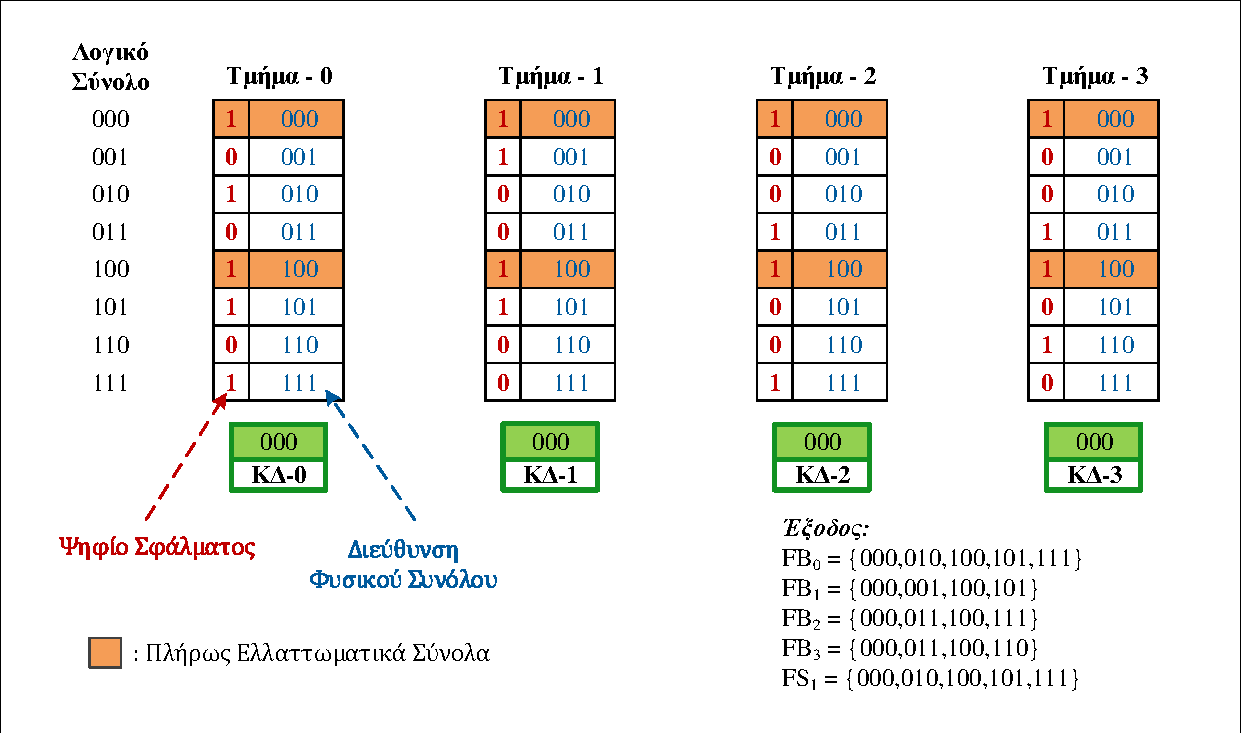
\includegraphics[width=\linewidth,trim=1cm 0.7cm 0.8cm 0.7cm, clip=true]{\algorithmsDIR/chap5_serial_example_step-0.pdf}}
    \caption{Αρχικοποίηση Σειριακού Αλγορίθμου}
    \label{fig:chap5_serial_init}
\end{figure}

Για την περιγραφή της μεθοδολογίας του σειριακού αλγορίθμου χρησιμοποιείται ένα παράδειγμα Πίνακα Πρόβλεψης Προορισμού Διακλάδωσης 4-τρόπων συνόλου συσχέτισης το οποίο παρουσιάζεται στο Σχήμα \ref{fig:chap5_serial_init}. Το πλήθος των σφαλμάτων δεν ανταποκρίνεται άμεσα στην πραγματικότητα αλλά διευκολύνει στην κατανόηση του τρόπου λειτουργίας του αλγορίθμου. Κάθε στοιχείο μιας στήλης του Σχήματος \ref{fig:chap5_serial_init} αποτελείται από δύο πεδία, το πρώτο υποδηλώνει εάν το πλαίσιο είναι ελαττωματικό ή όχι (1 ή 0 αντίστοιχα), ενώ το δεύτερο πεδίο υποδηλώνει τη φυσική διεύθυνση του πλαισίου. Όπως έχει ήδη αναφερθεί, η προτεινόμενη τεχνική υπολογίζει κατάλληλες τιμές για την επαναδιευθυνσιοδότηση των προσπελάσεων στον πίνακα, εκτελώντας την λογική πράξη \xor της αρχικής διεύθυνσης με μία τιμή μετάθεσης η οποία είναι αποθηκευμένη σε κατάλληλο καταχωρητή, δημιουργώντας έτσι τα λογικά σύνολα. Ένα λογικό σύνολο επομένως μπορεί να αποτελείται από ένα πλήθος πλαισίων είτε διαφορετικών είτε του ίδιου φυσικού συνόλου. Όταν οι τιμές των καταχωρητών είναι μηδενικές, τα λογικά και τα φυσικά σύνολα ταυτίζονται.
\par
Γνωρίζοντας τις θέσεις των ελαττωματικών πλαισίων κάθε τμήματος, στο βήμα της αρχικοποίησης καταγράφονται οι θέσεις αυτές σε τέσσερα διανύσματα αντίστοιχα: $FB_{0}$, $FB_{1}$, $FB_{2}$ και $FB_{3}$. Επίσης οι Καταχωρητές Διαμόρφωσης (ΚΔ) αρχικοποιούνται με τιμή 0, η οποία χρησιμοποιείται και στην κατάσταση κανονικής λειτουργίας όπου κανένα πλαίσιο δεν περιέχει ελαττωματικό δυαδικό ψηφίο. Επιπλέον, αρχικοποιείται το διάνυσμα $FS_{1}$ με τα περιεχόμενα του διανύσματος $FB_{0}$.

\begin{figure}[t]
    \centering
    \fbox{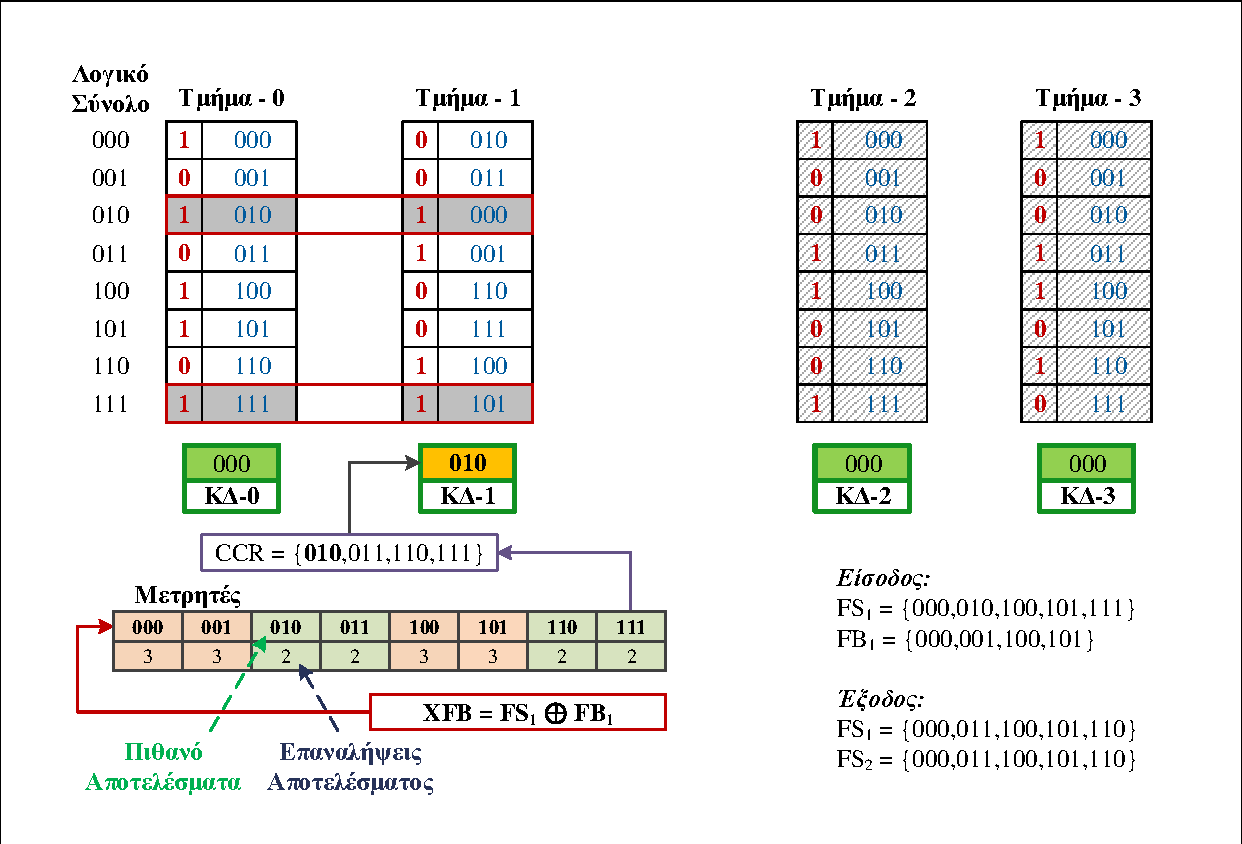
\includegraphics[width=\linewidth,trim=1cm 0.8cm 0.8cm 1cm, clip=true]{\algorithmsDIR/chap5_serial_example_step-1.pdf}}
    \caption{Σειριακό Βήμα 1\textsuperscript{ο} - Υπολογισμός ΚΔ-1}
    \label{fig:chap5_serial_step1}
\end{figure}

Στο πρώτο βήμα του αλγορίθμου, το οποίο παρουσιάζεται στο Σχήμα \ref{fig:chap5_serial_step1}, εκτελείται η συνάρτηση $XFB = FS_{1} \oplus FB_{1}$ για κάθε δυνατό συνδυασμό των περιεχομένων των δύο διανυσμάτων. Με τον υπολογισμό ενός αποτελέσματος γίνεται και η αύξηση του αντίστοιχου μετρητή. Κάθε μετρητής διατηρεί το ιστορικό εμφανίσεων ενός αποτελέσματος, όπως φαίνεται και στο Σχήμα \ref{fig:chap5_serial_step1}. Έτσι εάν το αποτέλεσμα της συνάρτησης είναι 0 η τιμή του μετρητής 0 αυξάνεται κατά ένα. Η πρώτη γραμμή του πίνακα μετρητών που παρουσιάζεται στο σχήμα περιέχει όλες τις δυνατές τιμές αποτελέσματος που μπορεί να πάρει η συνάρτηση:
\begin{equation}
    XFB = \{x \in \Re, 0 \leq x < 2^{log_2(\textit{πλήθος συνόλων})}\}
\end{equation}

Η δεύτερη γραμμή του πίνακα μετρητών περιέχει το άθροισμα των επαναλήψεων του αντίστοιχου αποτελέσματος, κατά τη διαδικασία εκτέλεσης των πράξεων \xor μεταξύ των στοιχείων των δύο διανυσμάτων. Συνεπώς, το άθροισμα των τιμών όλων των θέσεων της δεύτερης γραμμής πρέπει να ισούται με το γινόμενο του πλήθους των στοιχείων του πρώτου διανύσματος ($FS_{1}$) με το πλήθος των στοιχείων του δεύτερου διανύσματος ($FB_{1}$). Όσο δηλαδή ο συνολικός αριθμός λογικών πράξεων \xor που θα εκτελεστούν.
\par
Το πλήθος επαναλήψεων ενός αποτελέσματος, συνεπώς η τιμή του αντίστοιχου κελιού των μετρητών, υποδηλώνει πόσες περιπτώσεις θα παραμείνουν άλυτες μετά την εφαρμογή της συγκεκριμένης τιμής στον Καταχωρητή Διαμόρφωσης, δηλαδή πόσα λογικά σύνολα θα περιέχουν ελαττωματικά πλαίσια και στα δύο πρώτα τμήματα (Τμήμα-0 και Τμήμα-1). Επομένως, πρέπει να επιλεγεί η τιμή με το μικρότερο πλήθος επαναλήψεων.
\par
Από όλες τις δυνατές τιμές που μπορεί να λάβει ο \textit{ΚΔ-1}, επιλέγονται  αυτές με την ελάχιστη τιμή στον αντίστοιχο μετρητή. Οι επιλεγμένες τιμές αποθηκεύονται σε ένα διάνυσμα $CCR$ το οποίο δηλώνει τις εγκεκριμένες τιμές για τον καταχωρητή. Από τις τιμές που περιέχει το διάνυσμα $CCR$ επιλέγεται μία τυχαία η οποία αποθηκεύεται στον \textit{ΚΔ-1}. Σύμφωνα με τα περιεχόμενα των μετρητών του Σχήματος \ref{fig:chap5_serial_step1}, η καλύτερη λύση στο παρόν βήμα είναι η επιλογή μεταξύ των τιμών 010, 011, 110 και 111, ώστε να παραμείνουν δύο λογικά σύνολα με ελαττωματικά πλαίσια στο Τμήμα-0 και στο Τμήμα-1 ταυτόχρονα (για \textit{ΚΔ-1} = 010 $\Rightarrow$ λογικά σύνολα 010 και 111).
\par
Μετά την εφαρμογή της επιλεγμένης τιμής στον \textit{ΚΔ-1} εξάγονται δύο νέα διανύσματα. Το πρώτο διάνυσμα ($FS_{1}$) περιέχει τα σύνολα όπου μόνο ένα από τα δύο πλαίσια του λογικού συνόλου είναι ελαττωματικό, μεταξύ των δύο αυτών τμημάτων. Το δεύτερο διάνυσμα ($FS_{2}$) περιέχει τις θέσεις που και τα δύο πλαίσια είναι ελαττωματικά.

\begin{figure}[!b]
    \centering
    \fbox{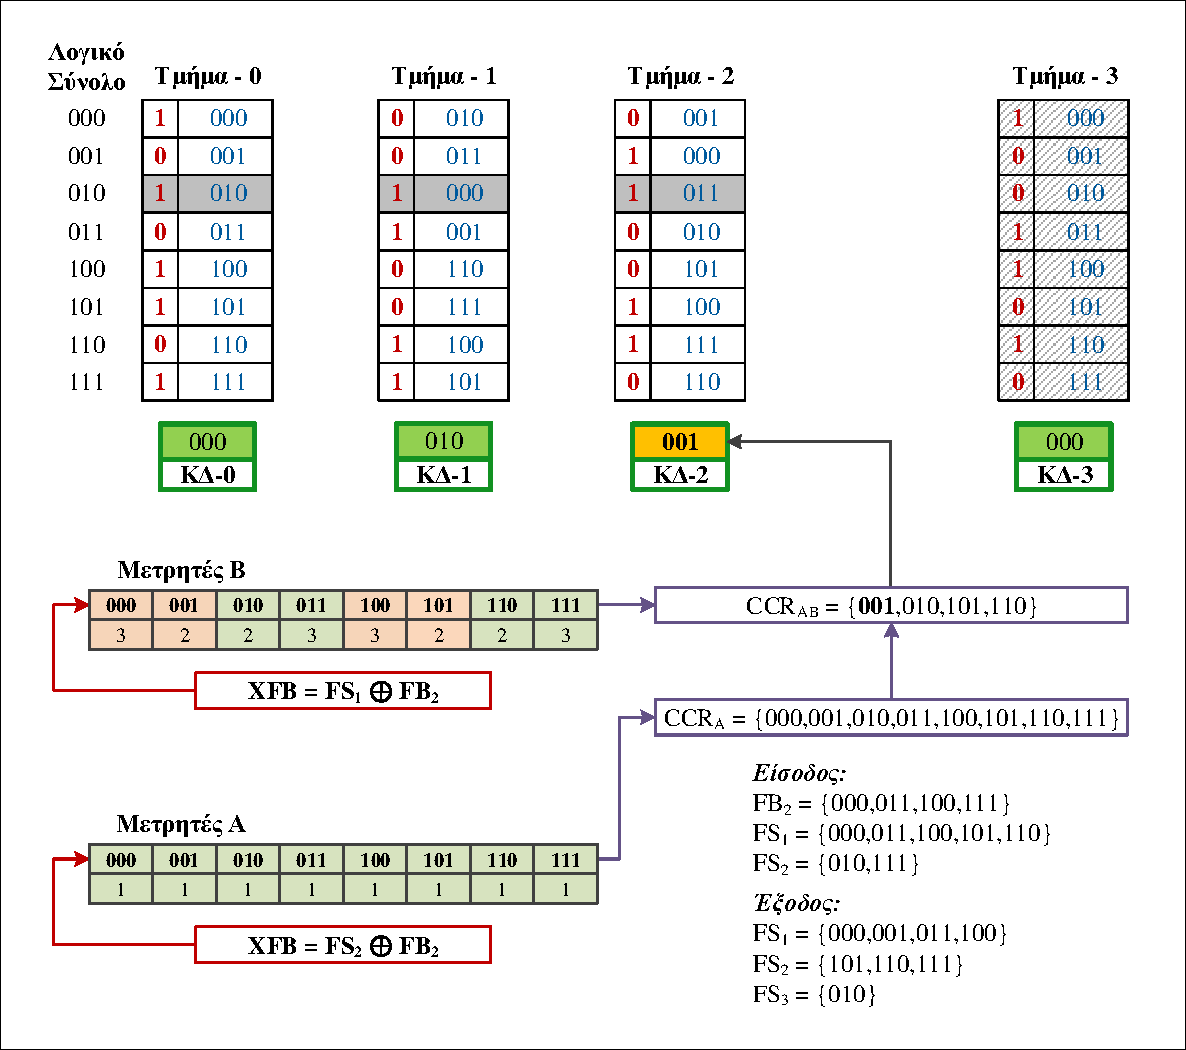
\includegraphics[width=\linewidth,trim=0.6cm 0.7cm 0.5cm 0.7cm, clip=true]{\algorithmsDIR/chap5_serial_example_step-2.pdf}}
    \caption{Σειριακό Βήμα 2\textsuperscript{ο} - Υπολογισμός ΚΔ-2}
    \label{fig:chap5_serial_step2}
\end{figure}

Κατά το δεύτερο βήμα, το οποίο παρουσιάζεται στο Σχήμα \ref{fig:chap5_serial_step2}, πρωταρχικός στόχος είναι η μείωση των λογικών συνόλων που θα περιέχουν 3 ελαττωματικά πλαίσια. Έτσι εκτελείται η συνάρτηση $XFB = FS_{2} \oplus FB_{2}$ για κάθε δυνατό συνδυασμό των περιεχομένων τους, καθώς και η αντίστοιχη αύξηση των μετρητών Α. Από όλες τις δυνατές τιμές που μπορεί να λάβει ο \textit{ΚΔ-2}, επιλέγονται αυτές με την ελάχιστη τιμή στον αντίστοιχο μετρητή. Οι επιλεγμένες αυτές τιμές αποθηκεύονται σε ένα διάνυσμα $CCR_{A}$.
\par
Δευτερεύων στόχος του αλγορίθμους σε αυτό το βήμα, είναι η μείωση των λογικών συνόλων που θα περιέχουν 2 ελαττωματικά πλαίσια. Για το λόγο αυτό, στη συνέχεια εκτελείται η συνάρτηση $XFB = FS_{1} \oplus FB_{2}$ με την αντίστοιχη ενημέρωση των μετρητών Β. Από τα στοιχεία που περιείχε το διάνυσμα $CCR_{A}$ επιλέγονται αυτά με τη μικρότερη τιμή στον πίνακα μετρητών Β. Τα επιλεγμένα στοιχεία αποθηκεύονται σε ένα διάνυσμα $CCR_{AB}$. Από το διάνυσμα αυτό επιλέγεται μία τιμή τυχαία η οποία αποθηκεύεται στον \textit{ΚΔ-2} (\textit{ΚΔ-2} = 001 στο παράδειγμα).
\par
Μετά την εφαρμογή της επιλεγμένης τιμής στον \textit{ΚΔ-2}, εξάγονται τρία νέα διανύσματα. Το πρώτο διάνυσμα ($FS_{1}$) περιέχει τα λογικά σύνολα που έχουν μόνο ένα από τα τρία πλαίσια ελαττωματικό, μεταξύ των τριών αυτών τμημάτων. Το δεύτερο διάνυσμα ($FS_{2}$) περιέχει τα σύνολα όπου δύο από τα τρία πλαίσια του λογικού συνόλου είναι ελαττωματικά. Το τρίτο διάνυσμα ($FS_{3}$) περιέχει τα σύνολα που και τα τρία πλαίσια είναι ελαττωματικά.

\begin{figure}[!b]
    \centering
    \fbox{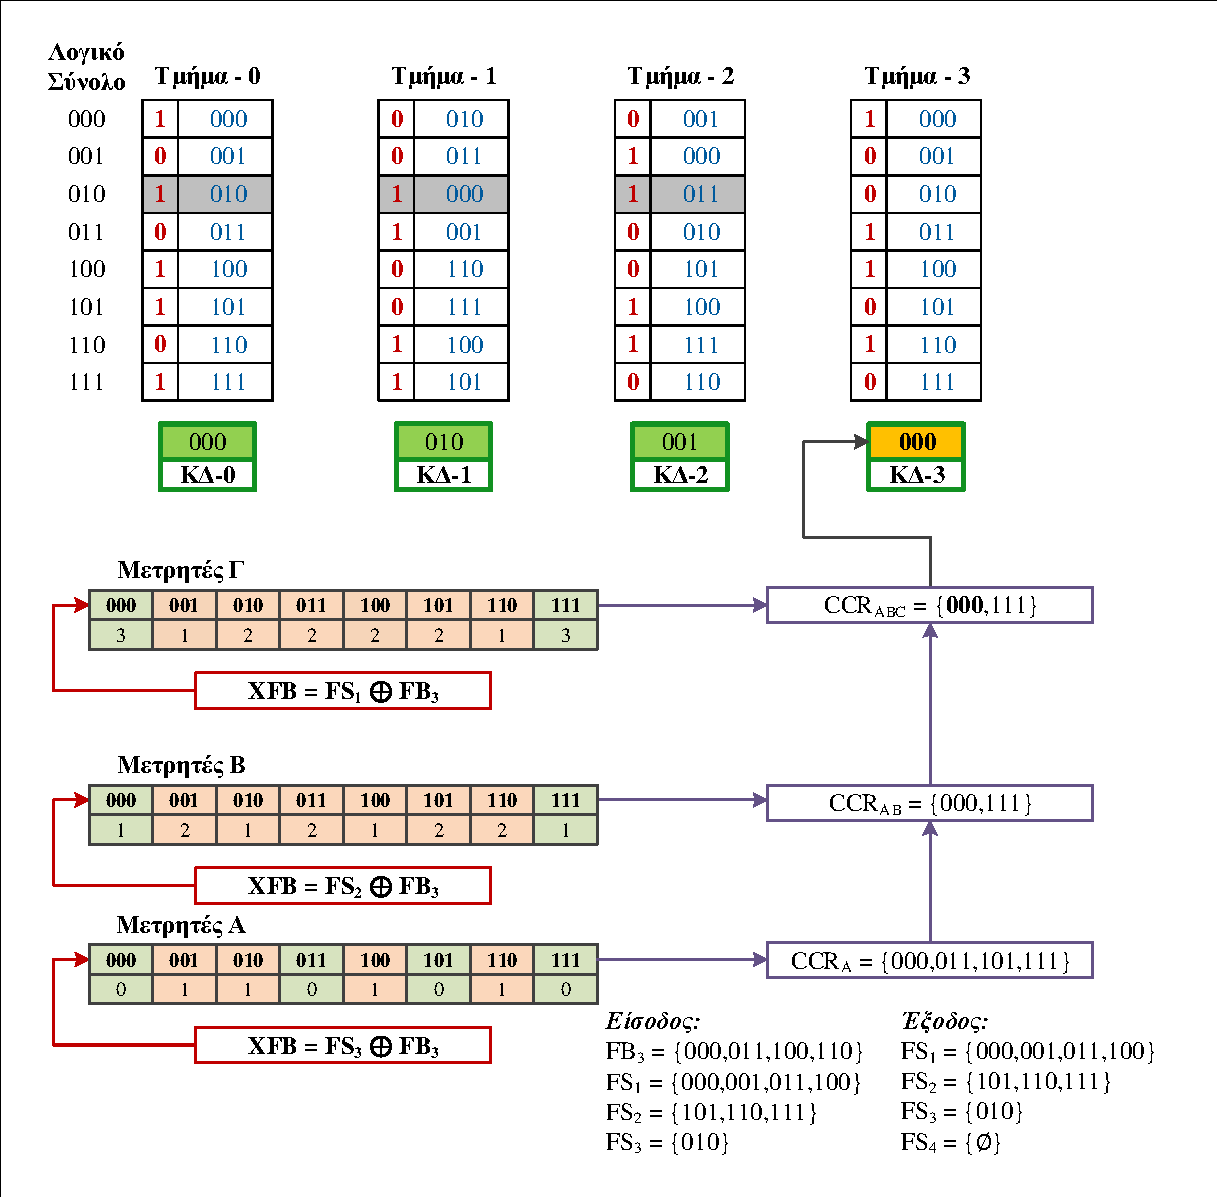
\includegraphics[width=\linewidth,trim=0.6cm 0.7cm 0.5cm 0.7cm, clip=true]{\algorithmsDIR/chap5_serial_example_step-3.pdf}}
    \caption{Σειριακό Βήμα 3\textsuperscript{ο} - Υπολογισμός ΚΔ-3}
    \label{fig:chap5_serial_step3}
\end{figure}

Κατά το τρίτο και τελευταίο βήμα, το οποίο παρουσιάζεται στο Σχήμα \ref{fig:chap5_serial_step3}, πρωταρχικός στόχος, ο οποίος αποτελεί και βασικό στόχο της προτεινόμενης τεχνικής, είναι η μείωση των λογικών συνόλων που θα περιέχουν 4 ελαττωματικά πλαίσια. Έτσι εκτελείται η συνάρτηση $XFB = FS_{3} \oplus FB_{3}$ για κάθε δυνατό συνδυασμό των περιεχομένων τους, με την αντίστοιχη αύξηση των μετρητών Α. Από όλες τις δυνατές τιμές που μπορεί να λάβει ο \textit{ΚΔ-3}, επιλέγονται αυτές με την ελάχιστη τιμή στον αντίστοιχο μετρητή και αποθηκεύονται σε ένα διάνυσμα $CCR_{A}$.
\par
Επόμενος στόχος του αλγορίθμους είναι η μείωση των λογικών συνόλων που θα περιέχουν 3 ελαττωματικά πλαίσια. Για το λόγο αυτό, εκτελείται η συνάρτηση $XFB = FS_{2} \oplus FB_{3}$ με την αντίστοιχη ενημέρωση των μετρητών Β. Από τα στοιχεία που περιείχε το διάνυσμα $CCR_{A}$ επιλέγονται αυτά με τη μικρότερη τιμή στον πίνακα μετρητών Β και αποθηκεύονται σε ένα νέο διάνυσμα $CCR_{AB}$.
\par
Τρίτος και με τη μικρότερη βαρύτητα στόχος του αλγορίθμους είναι η μείωση των λογικών συνόλων που θα περιέχουν 2 ελαττωματικά πλαίσια. Επομένως, εκτελείται η συνάρτηση $XFB = FS_{1} \oplus FB_{3}$ με την αντίστοιχη ενημέρωση των μετρητών Γ. Από τα στοιχεία που περιείχε το διάνυσμα $CCR_{AB}$ επιλέγονται αυτά με τη μικρότερη τιμή στον πίνακα μετρητών Γ και αποθηκεύονται σε ένα νέο διάνυσμα $CCR_{ABC}$. Από τις τιμές του διανύσματος αυτού επιλέγεται μία τυχαία η οποία αποθηκεύεται στον \textit{ΚΔ-3} (\textit{ΚΔ-3} = 000 στο παράδειγμα).
\par
Μετά την εφαρμογή της επιλεγμένης τιμής στον \textit{ΚΔ-3} εξάγονται τέσσερα νέα διανύσματα. Το πρώτο διάνυσμα ($FS_{1}$) περιέχει τα λογικά σύνολα όπου μόνο ένα από τα τέσσερα πλαίσια που το αποτελούν είναι ελαττωματικό. Το δεύτερο διάνυσμα ($FS_{2}$) τα λογικά σύνολα όπου δύο από τα τέσσερα πλαίσια είναι ελαττωματικά. Το τρίτο διάνυσμα ($FS_{3}$) τα λογικά σύνολα όπου τρία από τα τέσσερα πλαίσια είναι ελαττωματικά. Το τέταρτο διάνυσμα ($FS_{4}$) τα σύνολα όπου και τα τέσσερα πλαίσια είναι ελαττωματικά.
\par
Έπειτα από την εφαρμογή των νέων τιμών στους καταχωρητές διαμόρφωσης, όπως φανερώνεται και από το Σχήμα \ref{fig:chap5_serial_final}, τα πλήρως ελαττωματικά σύνολα έχουν εξαλειφθεί και η κατανομή των ελαττωματικών πλαισίων πλέον είναι πιο $``$δίκαιη$"$ μεταξύ των συνόλων.

\begin{figure}[h]
    \centering
    \fbox{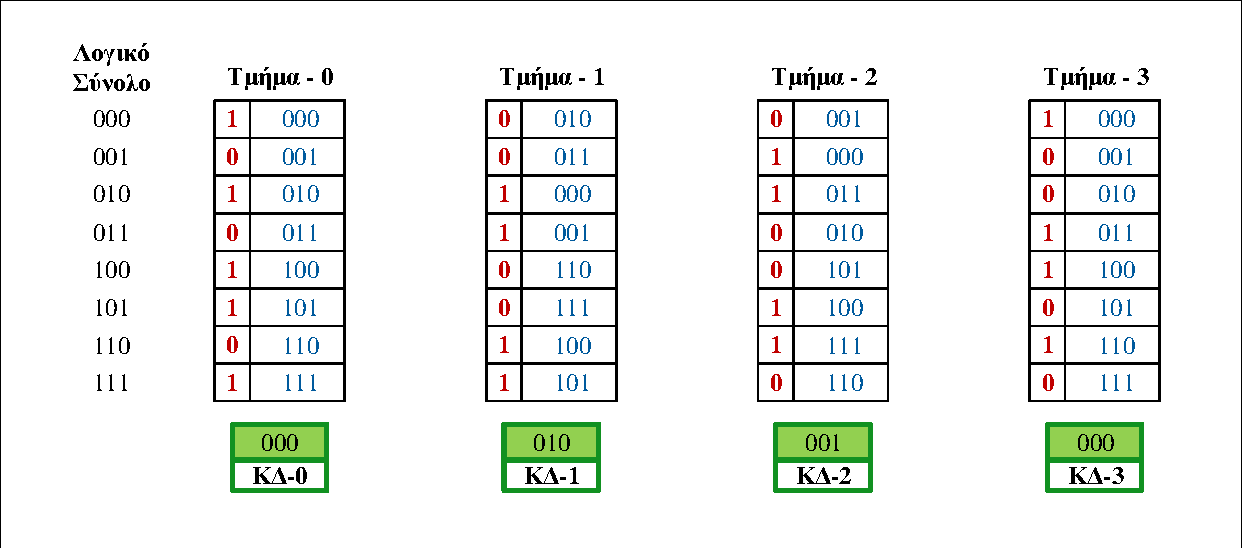
\includegraphics[width=\linewidth,trim=1cm 0.8cm 0.7cm 0.7cm, clip=true]{\algorithmsDIR/chap5_serial_example_step-final.pdf}}
    \caption{Λογικά σύνολα μετά την εκτέλεση του σειριακού αλγορίθμου}
    \label{fig:chap5_serial_final}
\end{figure}

%----------------------------------------------------------%

\subsection{Παράλληλος Αλγόριθμος}
\label{chap5_ParallelAlgorithm}

\begin{algorithm}[H]
    \captionsetup{}
    \caption{\ \ \ Παράλληλος Υπολογισμός Καταχωρητών Διαμόρφωσης}
    \label{alg:parallel}
    \begin{algorithmic}[1]
        \begin{footnotesize}
            \Statex 
            
            \Statex 
            \begin{center}
                \textit{\textbf{Περιγραφή Μεταβλητών και Συναρτήσεων}}
            \end{center}
            
            \Statex
            \begin{description}[leftmargin=9em,style=nextline]
                \item [$SetsNumber$] Πλήθος συνόλων
                \item [$WaysNumber$] Πλήθος τμημάτων
                \item [$FaultMaps$] Θέσεις σφαλμάτων στη μνήμη (διεύθυνση συνόλου, τμήμα)
                \item [$S$] Αποδεκτές τιμές Καταχωρητών Διαμόρφωσης
                \item [$FB_{w}$] Διευθύνσεις ελαττωματικών πλαισίων στο τμήμα - \en{w}
                \item [$XFB_{w}$] Διευθύνσεις ελαττωματικών πλαισίων στο τμήμα - \en{w} μετά την εφαρμογή της νέας τιμής στον Καταχωρητή Διαμόρφωσης - \en{w}
                \item [$FS_{[t,k]}$] Διευθύνσεις λογικών συνόλων με \en{k} ελαττωματικά πλαίσια, μεταξύ των τμημάτων που έχουν συμμετάσχει στο νήμα \en{t} έως το τρέχον βήμα του αλγορίθμου
                \item [$CCR$] Υποψήφιες τιμές του ελεγχόμενου Καταχωρητή Διαμόρφωσης μετά από κάθε βήμα του αλγορίθμου
                \item [$CR_{w}$] Τελική τιμή του Καταχωρητή Διαμόρφωσης - \en{w}
                \item [$COUNTER{[X,Y]}$] Μετρητές επανάληψης αποτελεσμάτων \en{Y} των λογικών πράξεων \xor. Κάθε γραμμή του πίνακα έχει διαφορετική βαρύτητα. Η ανώτερη γραμμή (μικρότερη τιμή του \en{X}) έχει τη μικρότερη βαρύτητα, ενώ η κατώτερη γραμμή (μεγαλύτερη τιμή του \en{X}) τη μεγαλύτερη βαρύτητα, στην επιλογή τιμών για τους Καταχωρητές Διαμόρφωσης.\\
                ($Y=0 \Rightarrow COUNTER[X,0]++$)
                \item[$elements(A)$] Συνάρτηση εύρεσης πλήθους στοιχείων του διανύσματος \en{A}
                \item[$minimum(A)$] Συνάρτηση εύρεσης μικρότερου στοιχείου του διανύσματος \en{A}
                \item[$random(A)$] Συνάρτηση τυχαίας επιλογής στοιχείου από το διάνυσμα \en{A}
            \end{description}
            
            \begin{center}
                \hrulefill
            \end{center}
            
            \selectlanguage{english}
            \Procedure {ParallelPermutation}{$SetsNumber$, $WaysNumber$, $FaultMaps$}
                \State \Comment {\gr{Αρχικοποίησης}}
                \State $ maxAddress = SetsNumber - 1 $;
                \State $ S = \{ x\in \mathbb{R}, 0\le x\le maxAddress \} $;
                \State $parallelSteps = log2(WaysNumber) - 1$;
                \State $threadsNumber = WaysNumber$;
                
                \\
                \For {$w = 0$ to $WaysNumber - 1$}
                    \State $ FB_{w} = \{ \textit{\gr{ελαττωματικά πλαίσια τμήματος}-w} \} $;
                    \State $ XFB_{w} = \{ \emptyset \} $;
                    \State $ CR_{w} = 0 $;
                \EndFor
                \For {$b = 0$ to $WaysNumber$}
                    \State $ FS_{[w,b]} = \{ \emptyset \} $;
                \EndFor
                
                \\
                \State \linecomment{\gr{Αρχικά τα σύνολα του νήματος} k \gr{με 1 ελαττωματικό πλαίσιο ταυτίζονται με αυτά του τμήματος} k}
                \State $ FS_{w,1} =  FB_{w} $;
                \State $ FS_{w,0} =  S - FS_{w,1} $;
                
                %continue on next page
                \algstore{parallel_alg_part1}
        \end{footnotesize}
    \end{algorithmic}
\end{algorithm}

\begin{algorithm}[H]
    \ContinuedFloat
    \caption{\ \ \ Παράλληλος Υπολογισμός Καταχωρητών Διαμόρφωσης (Συνέχεια)}
    \begin{algorithmic}[1]
        \algrestore{parallel_alg_part1}
        \begin{footnotesize}
            \selectlanguage{english}
                \State \Comment {\gr{Βήματα υπολογισμού κατάλληλης τιμής για κάθε καταχωρητή} w}
                
                \For {$pstep = 1$ to $parallelSteps$}
                    \State $ threadWays = WaysNumber/threads $;
                    \linecomment{\gr{πλήθος τμημάτων ανά νήμα}}
                    
                    \\
                    \State \linecomment{\gr{Εκτέλεση συνάρτησης} XOR \gr{μεταξύ των νημάτων} t \gr{και} t+1. \gr{Η τιμή που εξάγεται}}
                    \State \linecomment{\gr{μεταβάλει τις τιμές των καταχωρητών των τμημάτων που περιέχει το νήμα} t+1.}
                    \For {$t = 0$ to $threadsNumber$ step $2$}
                        \State $ COUNTER\left[0 : 2*threadWays, 0 : maxAddress \right] = 0 $;
                        
                        \\
                        \For {$i = threadWays$ to $1$ step $-1$}
                            \For {$j = threadWays$ to $1$ step $-1$}
                                \State $ X = i + j $;
                                \ForAll{$F_{R}$ in $FS_{[t,i]}$}
                                    \ForAll{$F_{L}$ in $FS_{[t+1,j]}$}
                                        \State $ Y = F_{L} \oplus F_{R} $;
                                        \State $ COUNTER\left[N, Y \right] = COUNTER\left[X, Y \right] + 1 $;
                                    \EndFor
                                \EndFor
                            \EndFor
                        \EndFor
                        
                        \\
                        \State \linecomment{\gr{Υπολογισμός του συνόλου υποψήφιων τιμών, κρατώντας σε κάθε επανάληψη αυτές}}
                        \State \linecomment{\gr{με την ελάχιστη τιμή στη γραμμή} X \gr{του πίνακα. Η αναζήτηση ξεκινάει από την}}
                        \State \linecomment{\gr{κατώτερη γραμμή η οποία έχει τη μεγαλύτερη βαρύτητα (στόχος είναι η μείωση}}
                        \State \linecomment{\gr{των συνόλων που περιέχουν πολλά ελαττωματικά πλαίσια).}}
                        \State $ CCR = S $;
                        \For {$X = 2*threadWays$ to $2$ step $-1$}
                            \If {$ elements(CCR) > 1 $}
                                
                                \\
                                \State $ CAND\_CNT = \{ \emptyset \} $;
                                \ForAll{$CR$ in $CCR$}
                                    \State $ CAND\_CNT = CAND\_CNT \cup COUNTER\left[X, CR \right] $;
                                \EndFor
                                \State $ MIN\_CNT = minimum(CAND\_CNT) $;
                                \State $ NEW\_CCR = \{ \emptyset \} $;
                                \ForAll{$CR$ in $CCR$}
                                    \If {$ COUNTER\left[X, CR \right] = MIN\_CNT$}
                                        \State $ NEW\_CCR = NEW\_CCR \cup CR $;
                                    \EndIf
                                \EndFor
                                
                                \\
                                \State $ CCR = NEW\_CCR $;
                            \EndIf
                        \EndFor
                        
                        \\
                        \State $ TCR = random(CCR) $;
                        \For {$w = (t+1)*threadWays$ to $(t+2)*threadWay - 1$}
                            \State $ CR_{w} = CR_{w} \oplus TCR $;
                        \EndFor
                %continue on next page
                \algstore{parallel_alg_part2}
        \end{footnotesize}
    \end{algorithmic}
\end{algorithm}

\begin{algorithm}[H]
    \ContinuedFloat
    \caption{\ \ \ \gr{Παράλληλος Υπολογισμός Καταχωρητών Διαμόρφωσης (Συνέχεια)}}
    \begin{algorithmic}[1]
        \algrestore{parallel_alg_part2}
        \begin{footnotesize}
            \selectlanguage{english}
                        \For {$w = threadWays$ to $0$ step $-1$}
                            \State $ XFS = \{ \emptyset \} $;
                            \ForAll{$F$ in $FS_{[t+1,w]}$}
                                \State $ XFS = XFS \cup (F \oplus TCR) $;
                            \EndFor
                            $ FS_{[t+1,w]} = XFS $
                        \EndFor
                    \EndFor
                    \ \linecomment{t = t + 2}
                    
                    \\
                    \For {$t = 0$ to $threadsNumber$ step $2$}
                        \For {$w = 2*threadWays$ to $0$ step $-1$}
                            \State $ NFS = \{ \emptyset \} $;
                        \EndFor
                    
                        \For {$i = threadWays$ to $0$ step $-1$}
                            \For {$j = threadWays$ to $0$ step $-1$}
                                \State $ X = i + j $;
                                \State $ NFS_{X} = NFS_{X} \cup (FS_{[t,i]} \cap FS_{[t+1,j]}) $;
                            \EndFor
                        \EndFor
                        
                        \For {$w = 2*threadWays$ to $1$ step $-1$}
                            $ FS_{[t/2,w]} = NFS_{w} $
                        \EndFor
                    \EndFor
                    
                    \State $threadsNumber = threadsNumber/2 $;
                    
                \EndFor
                \ \linecomment{pstep = pstep + 1}
                
                \For {$w = 0$ to $WaysNumber$}
                    \ForAll{$F$ in $FB_{w}$}
                        \State $ XFB_{w} = XFB_{w} \cup (F \oplus CR_{w}) $;
                    \EndFor
                \EndFor
            \EndProcedure
        \end{footnotesize}
    \end{algorithmic}
\end{algorithm}

\clearpage

\subsubsection*{Παράδειγμα}

\begin{figure}[t]
    \centering
    \fbox{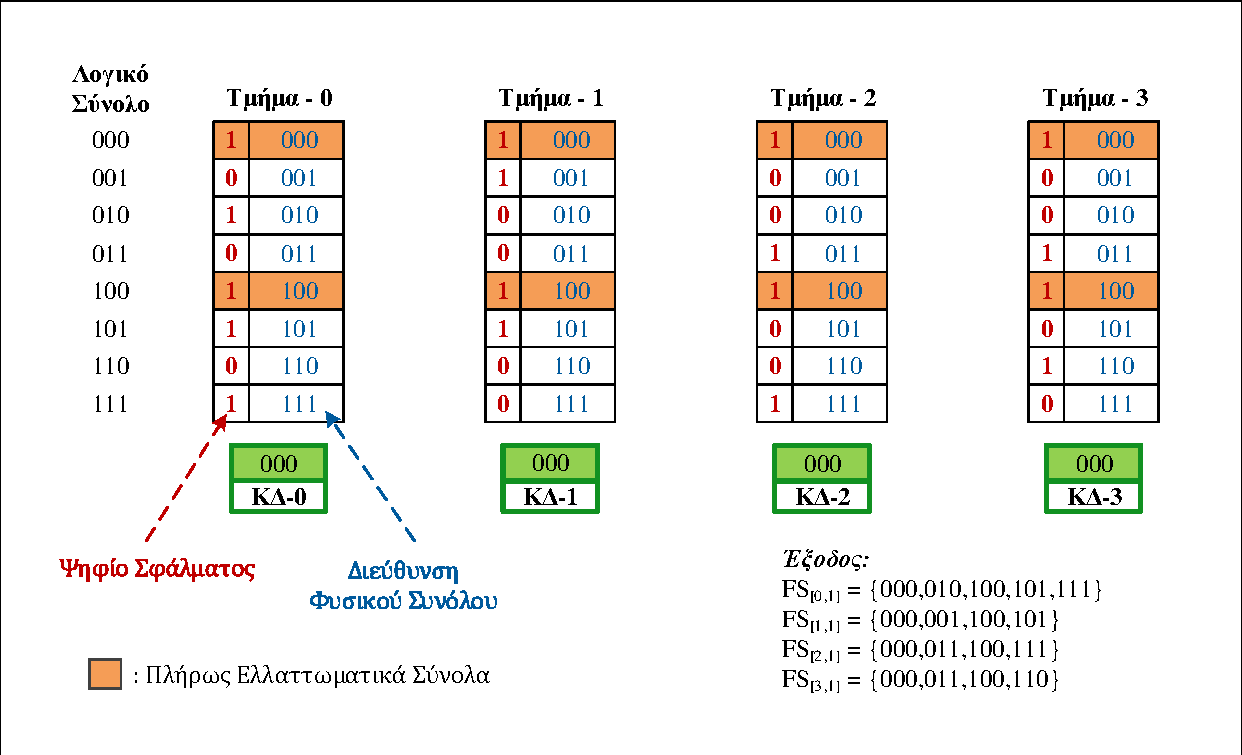
\includegraphics[width=\linewidth,trim=1cm 1cm 0.8cm 1cm, clip=true]{\algorithmsDIR/chap5_parallel_example_step-0.pdf}}
    \caption{Αρχικοποίηση Παράλληλου Αλγορίθμου}
    \label{fig:chap5_parallel_init}
\end{figure}

Για το παράδειγμα Πίνακα Πρόβλεψης Προορισμού Διακλάδωσης του σειριακού αλγορίθμου, αυτή τη φορά χρησιμοποιείται ο παράλληλος αλγόριθμος για τον υπολογισμό κατάλληλων τιμών των Καταχωρητών Διαμόρφωσης. Σε αντιστοιχία με τον σειριακό αλγόριθμο, κατά την αρχικοποίηση καταγράφονται οι θέσεις των ελαττωματικών πλαισίων των τεσσάρων τμημάτων στα αντίστοιχα διανύσματα: $FB_{0}$, $FB_{1}$, $FB_{2}$ και $FB_{3}$. Επίσης οι καταχωρητές αρχικοποιούνται με τιμή 0, όπως φανερώνει και το Σχήμα \ref{fig:chap5_parallel_init}.
\par
Θεωρώντας πως αρχικά κάθε τμήμα πλαισίων αντιστοιχεί σε ένα νήμα, ο αλγόριθμος υπολογισμού αποτελείται από στάδια παραλληλοποίησης όπου σε κάθε ένα από αυτά εκτελείται η συνάρτηση \xor μεταξύ δύο γειτονικών νημάτων. Στο τέλος της εκτέλεσης του σταδίου, γίνεται συνένωση των γειτονικών νημάτων σε ένα νέο νήμα (τα τ και τ+1 νήματα συνενώνονται). Στο επόμενο στάδιο ακολουθείται η ίδια διαδικασία για τα νέα μεγαλύτερα νήματα. Για κάθε νήμα εξάγονται κατάλληλα διανύσματα $FS_{[\mathgr{νήμα,ελαττωματικά πλαίσια συνόλου}]}$ που δηλώνουν τα λογικά σύνολα με τον αντίστοιχο αριθμό ελαττωματικών πλαισίων εντός του νήματος. Έτσι αρχικά για τα διανύσματα θα ισχύει: $FS_{[0,1]} = FB_{0}$, $FS_{[1,1]} = FB_{1}$, $FS_{[2,1]} = FB_{2}$ και $FS_{[3,1]} = FB_{3}$, όπως αναφέρεται και στο Σχήμα \ref{fig:chap5_parallel_init}.

\begin{figure}[t]
    \centering
    \fbox{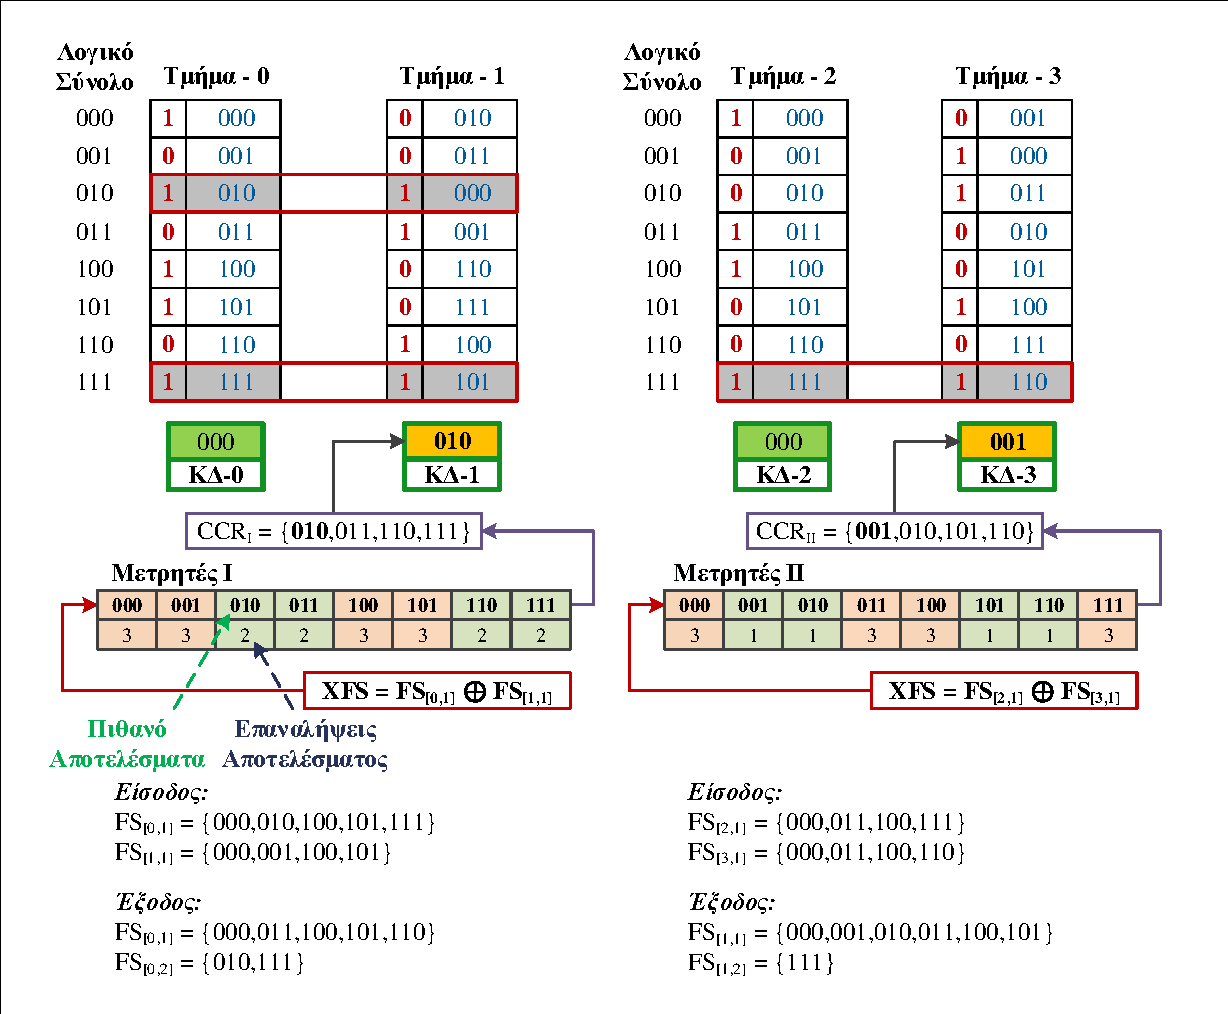
\includegraphics[width=\linewidth,trim=0.8cm 0.6cm 0.8cm 0.7cm, clip=true]{\algorithmsDIR/chap5_parallel_example_step-1.pdf}}
    \caption{Παράλληλο Βήμα 1\textsuperscript{ο} - Υπολογισμός ΚΔ-1 και KΔ-3}
    \label{fig:chap5_parallel_step1}
\end{figure}

Στο πρώτο βήμα του αλγορίθμου, εκτελούνται παράλληλα οι συναρτήσεις  $XFS = FS_{[0,1]} \oplus FS_{[1,1]}$  και $XFS = FS_{[2,1]} \oplus FS_{[3,1]}$, για κάθε δυνατό συνδυασμό των περιεχομένων των διανυσμάτων $FS$. Με την εκτέλεση κάθε πράξης γίνεται και η αύξηση του κατάλληλου μετρητή του αντίστοιχου ζεύγους νημάτων (μετρητές Ι και ΙΙ). Κάθε μετρητής διατηρεί το ιστορικό εμφανίσεων του αντίστοιχου αποτελέσματος, όπως φαίνεται και στο Σχήμα \ref{fig:chap5_parallel_step1}. Ακολουθώντας τη λογική του σειριακού αλγορίθμου, η δεύτερη γραμμή του πίνακα μετρητών περιέχει το πλήθος επαναλήψεων της αντίστοιχης τιμής ως αποτέλεσμα των λογικών συναρτήσεων \xor που εκτελούνται μεταξύ δύο γειτονικών τμημάτων (Τμήμα-0/Τμήμα-1 και Τμήμα-2/Τμήμα-3). Η τιμή μίας θέσης υποδηλώνει τον αριθμό των λογικών συνόλων που και στα δύο τμήματα τα πλαίσια που τα αποτελούν είναι ελαττωματικά, όταν στον Καταχωρητή Διαμόρφωσης του δεύτερου τμήματος κάθε ζεύγους νημάτων εφαρμοστεί η τιμή αυτή (\textit{ΚΔ-1} και \textit{ΚΔ-3} αντίστοιχα).
\par
Επομένως, από όλες τις δυνατές τιμές που μπορούν να λάβουν οι \textit{ΚΔ-1} και \textit{ΚΔ-3} επιλέγονται αυτές με την ελάχιστη τιμή στον αντίστοιχο μετρητή. Οι επιλεγμένες αυτές τιμές αποθηκεύονται στα διανύσματα $CCR_{I}$ και $CCR_{II}$. Από τα περιεχόμενα αυτών των διανυσμάτων, επιλέγεται μία τιμή τυχαία από κάθε ένα, η οποία αποθηκεύεται στους \textit{ΚΔ-1} και \textit{ΚΔ-3} αντίστοιχα (\textit{ΚΔ-1} = 010 και \textit{ΚΔ-3} = 001 στο παράδειγμα).
\par
Μετά την εφαρμογή της επιλεγμένης τιμής στους \textit{ΚΔ-1} και \textit{ΚΔ-3} εξάγονται δύο νέα διανύσματα για κάθε ζεύγος νημάτων. Το πρώτο διάνυσμα ($FS_{[0,1]}$ και $FS_{[1,1]}$ αντίστοιχα) περιέχει τις θέσεις όπου μόνο ένα από τα δύο πλαίσια είναι ελαττωματικό, μεταξύ των δύο τμημάτων που θα αποτελούν το νέο ενοποιημένο νήμα. Το δεύτερο διάνυσμα ($FS_{[0,2]}$ και $FS_{[1,2]}$ αντίστοιχα) περιέχει τις θέσεις όπου και τα δύο πλαίσια είναι ελαττωματικά.

\begin{figure}[!t]
    \centering
    \fbox{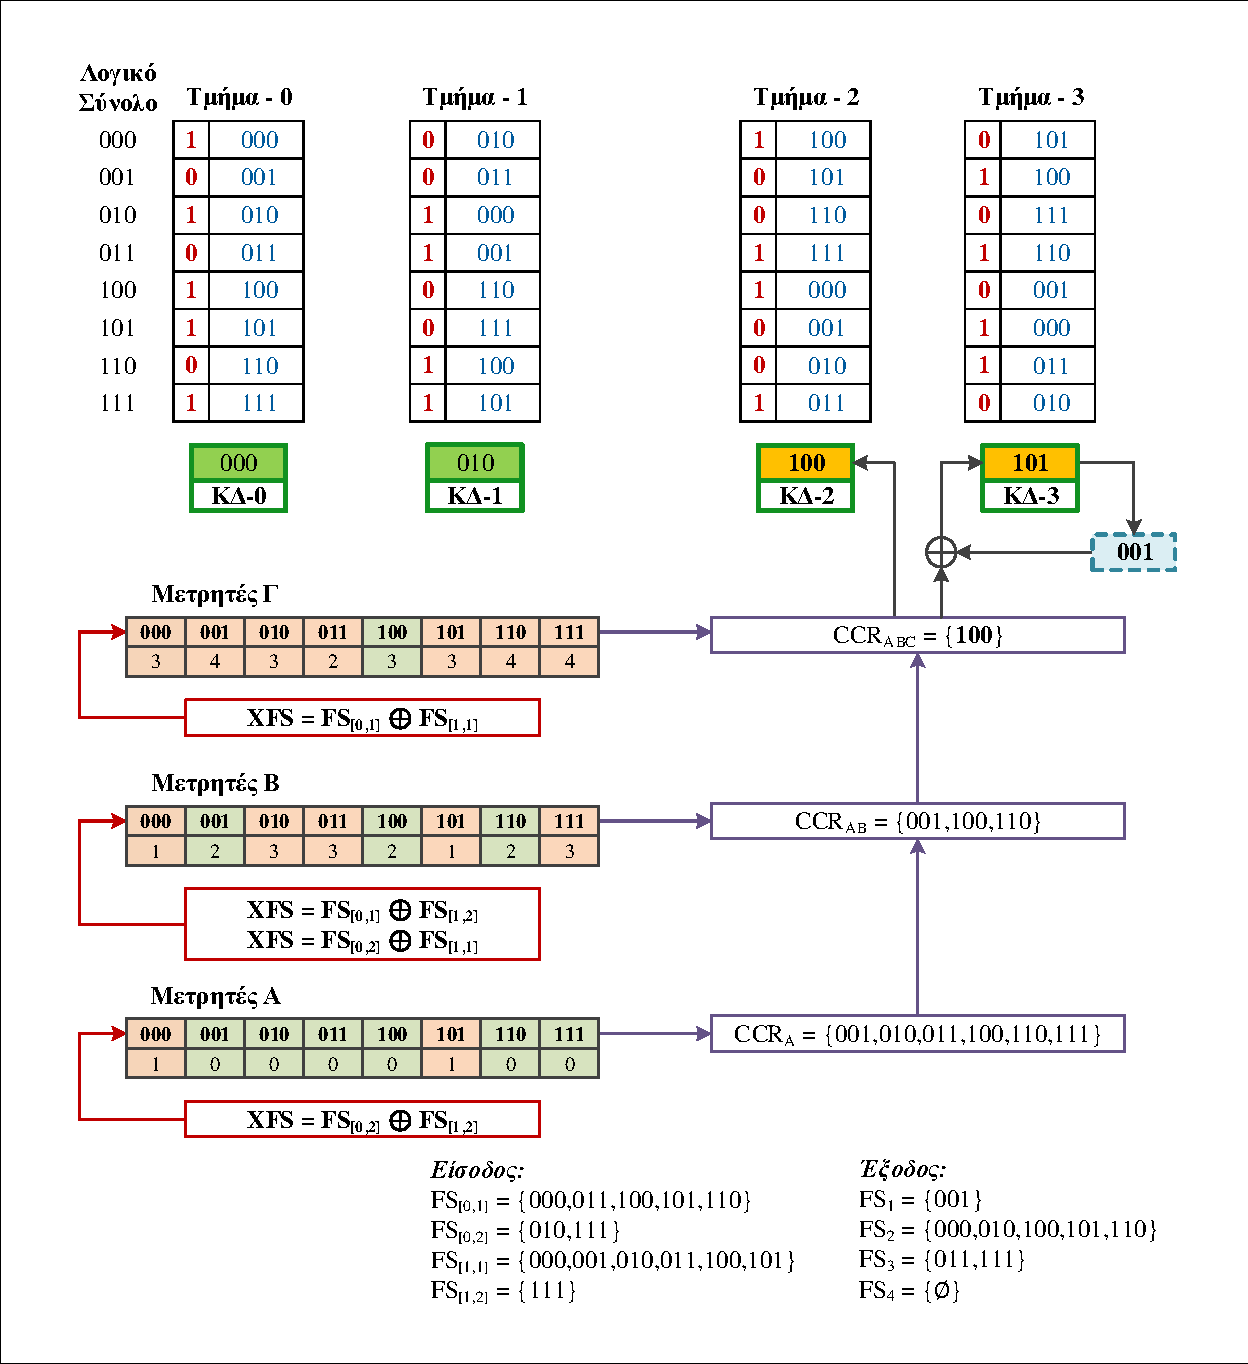
\includegraphics[width=\linewidth,trim=1cm 1cm 1cm 1cm, clip=true]{\algorithmsDIR/chap5_parallel_example_step-2.pdf}}
    \caption{Παράλληλο Βήμα 2\textsuperscript{ο} - Υπολογισμός ΚΔ-2 και ενημέρωση KΔ-3}
    \label{fig:chap5_parallel_step2}
\end{figure}

Κατά το δεύτερο βήμα, το οποίο απεικονίζεται στο Σχήμα \ref{fig:chap5_parallel_step2}, γίνεται ο υπολογισμός κατάλληλης τιμής του \textit{ΚΔ-2} και ενημέρωση του \textit{ΚΔ-3}. Κύριο στόχο αποτελεί η μείωση των λογικών συνόλων που θα περιέχουν 4 ελαττωματικά πλαίσια, συνεπώς εκτελείται η συνάρτηση $XFS = FS_{[0,2]} \oplus FS_{[1,2]}$ για κάθε δυνατό συνδυασμό των περιεχομένων αυτών των διανυσμάτων, καθώς και η αντίστοιχη αύξηση των μετρητών Α. Από όλες τις δυνατές τιμές που μπορεί να λάβει ο \textit{ΚΔ-2} επιλέγονται αυτές με την ελάχιστη τιμή στον αντίστοιχο μετρητή. Οι επιλεγμένες τιμές αποθηκεύονται σε ένα διάνυσμα $CCR_{A}$.
\par
Εφόσον έχει εξασφαλιστεί στο μέγιστο δυνατό η επίλυση του πρώτου στόχου, ο αλγόριθμος αναζητά και τη μείωση των λογικών συνόλων που θα περιέχουν 3 ελαττωματικά πλαίσια. Για το λόγο αυτό εκτελούνται οι συναρτήσεις $XFS = FS_{[0,1]} \oplus FS_{[1,2]}$ και $XFS = FS_{[0,2]} \oplus FS_{[1,1]}$ με κατάλληλη ενημέρωση των κοινών μετρητών Β. Από τα στοιχεία που περιείχε το διάνυσμα $CCR_{A}$ επιλέγονται αυτά με τη μικρότερη τιμή στον πίνακα μετρητών Β και αποθηκεύονται σε ένα νέο διάνυσμα $CCR_{AB}$.
\par
Έχοντας ολοκληρώσει τους δύο πρώτους στόχους, ο αλγόριθμος ελέγχει τη δυνατότητα μείωσης των λογικών συνόλων που θα περιέχουν 2 ελαττωματικά πλαίσια. Ο έλεγχος αυτός γίνεται μέσω της εκτέλεσης της συνάρτησης $XFS = FS_{[0,1]} \oplus FS_{[1,1]}$ με την αντίστοιχη ενημέρωση των μετρητών Γ. Από τα στοιχεία που περιείχε το διάνυσμα $CCR_{AB}$ επιλέγονται αυτά με τη μικρότερη τιμή στον πίνακα μετρητών Γ και αποθηκεύονται σε ένα νέο διάνυσμα $CCR_{ABC}$.
\par
Από τις τιμές που θα καταλήξουν στο διάνυσμα $CCR_{ABC}$ επιλέγεται μία τυχαία, η οποία γίνεται \xor με τις προηγούμενες τιμές των \textit{ΚΔ-2} και \textit{ΚΔ-3} και τα αποτελέσματά των συναρτήσεων αποθηκεύονται στους αντίστοιχους Καταχωρητές Διαμόρφωσης. Έτσι θα έχουμε τις νέες τιμές \textit{ΚΔ-2’ = ΚΔ-2} $\oplus$ $CCR$ και \textit{ΚΔ-3’ = ΚΔ-3} $\oplus$ $CCR$ (\textit{ΚΔ-2} = 100 και \textit{ΚΔ-3} = 101 στο παράδειγμα).
\par
Μετά την εφαρμογή των επιλεγμένων τιμών στους \textit{ΚΔ-2} και \textit{ΚΔ-3}, εξάγονται τέσσερα νέα διανύσματα. Το πρώτο διάνυσμα ($FS_{1}$) περιέχει τα λογικά σύνολα όπου μόνο ένα από τα τέσσερα πλαίσια είναι ελαττωματικό. Το δεύτερο διάνυσμα ($FS_{2}$) τα λογικά σύνολα όπου δύο από τα τέσσερα πλαίσια είναι ελαττωματικά. Το τρίτο διάνυσμα ($FS_{3}$) τα λογικά σύνολα όπου τρία από τα τέσσερα πλαίσια είναι ελαττωματικά. Το τέταρτο διάνυσμα ($FS_{4}$) τα λογικά σύνολα όπου και τα τέσσερα πλαίσια είναι ελαττωματικά.
\par
Με την εφαρμογή των νέων τιμών στους καταχωρητές διαμόρφωσης, όπως φανερώνει και το Σχήμα \ref{fig:chap5_parallel_final}, το αποτέλεσμα είναι παρόμοιο με τον σειριακό αλγόριθμο καθώς τα πλήρως ελαττωματικά σύνολα έχουν εξαλειφθεί.

\begin{figure}[h]
    \centering
    \fbox{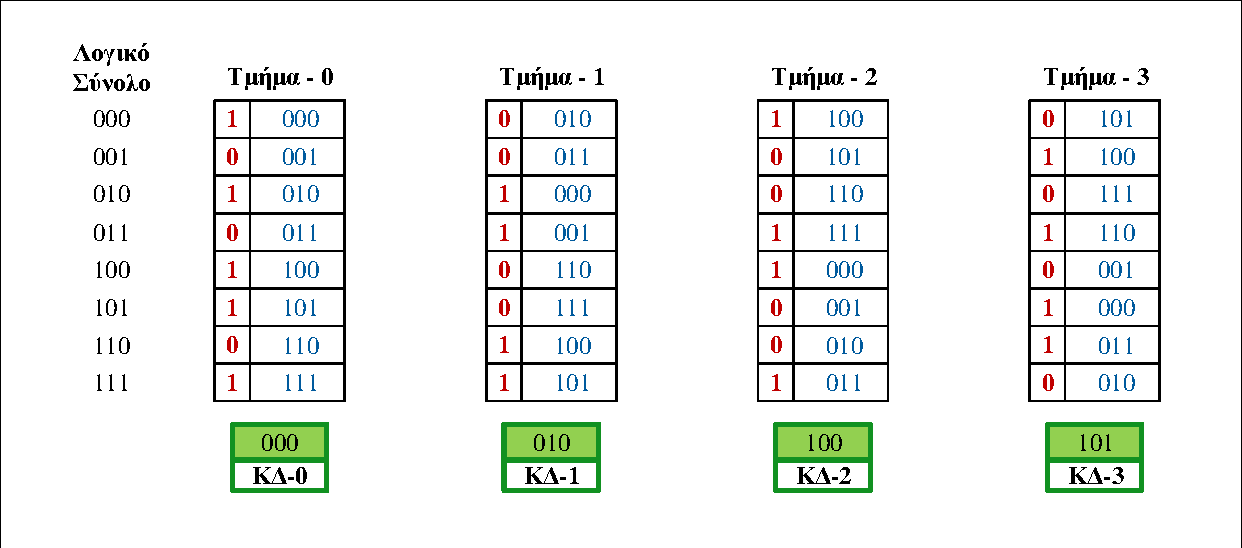
\includegraphics[width=\linewidth,trim=1cm 0.8cm 0.7cm 0.7cm, clip=true]{\algorithmsDIR/chap5_parallel_example_step-final.pdf}}
    \caption{Λογικά σύνολα μετά την εκτέλεση του παράλληλου αλγορίθμου}
    \label{fig:chap5_parallel_final}
\end{figure}

%----------------------------------------------------------%

\section{Βελτιστοποίηση}
\label{chap5_ImprovedMethod}

Όπως θα αποδειχθεί και από την πειραματική αξιολόγηση της τεχνικής που πραγματοποιείται στην Ενότητα \ref{chap5_AlgorithmResults}, ο τρόπος λειτουργίας της προτεινόμενης τεχνικής σε συνδυασμό με την τυχαιότητα των θέσεων των ελαττωματικών κυψελίδων, σε ορισμένες περιπτώσεις καθιστά αδύνατη την ολοκληρωτική εξάλειψη των πλήρως ελαττωματικών συνόλων. Στη μορφή της τεχνικής που παρουσιάστηκε έως τώρα η διεύθυνση προσπέλασης σε κάθε τμήμα πλαισίων μεταβάλετε από έναν και μόνο καταχωρητή. Το γεγονός αυτό δεν επιτρέπει την διαφοροποίηση του τρόπου μετάθεσης μεταξύ τμημάτων των τμημάτων. Για παράδειγμα, ένας επιθυμητός τρόπος μεταβολής της διεύθυνσης στο Τμήμα-0 θα μπορούσε να είναι ο ακόλουθος:
\begin{enumerate}[itemsep=0.5pt]
    \item Σύνολα 000 έως 011 $\Longrightarrow$ \xor με την τιμή 010
    \item Σύνολα 100 έως 111 $\Longrightarrow$ \xor με την τιμή 001
\end{enumerate}

Η λύση για την επίτευξη αυτού του αποτελέσματος έρχεται από τη διάσπαση των τμημάτων πλαισίων σε υποτμήματα, με τη χρήση περισσότερων Καταχωρητών Διαμόρφωσης ανά τμήμα, όπως παρουσιάζεται στο Σχήμα \ref{fig:chap5_multiCR_init}, για το παράδειγμα του σειριακού αλγορίθμου.

\begin{figure}[!t]
    \centering
    \fbox{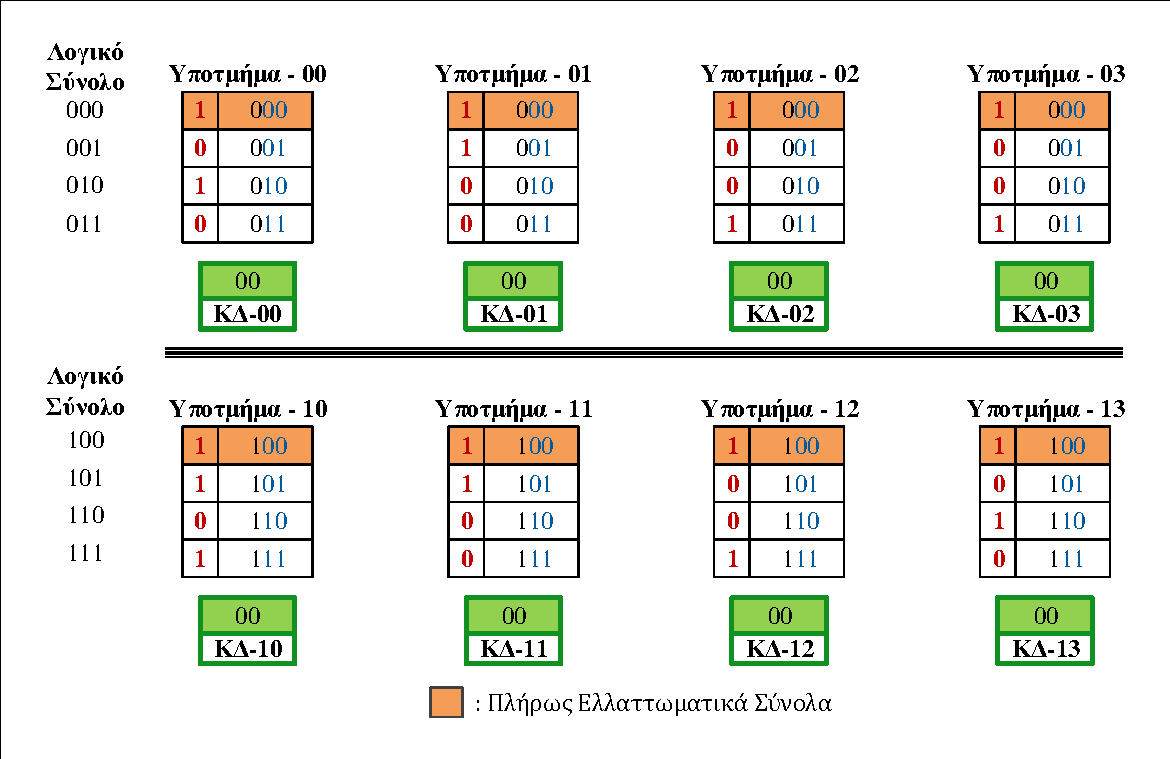
\includegraphics[width=\linewidth,trim=0.5cm 0.7cm 0.5cm 0.7cm, clip=true]{\algorithmsDIR/chap5_multiCR_example_step-0.pdf}}
    \caption{Μορφή βελτιστοποιημένης τεχνικής}
    \label{fig:chap5_multiCR_init}
\end{figure}

Κάθε Υποτμήμα-Χ αποτελείται από ένα πλήθος Πλαισίων-Χ συνεχόμενων συνόλων και διαθέτει ξεχωριστό Καταχωρητή Διαμόρφωσης. Επομένως, στο παράδειγμα του σχήματος όπου ο Πίνακας Πρόβλεψης Προορισμού Διακλάδωσης αποτελείται από 4 τμήματα με 2 υποτμήματα το κάθε ένα, ο συνολικός αριθμός απαιτούμενων καταχωρητών είναι 8 ($4\times2$). Ο αλγόριθμος για τον υπολογισμό τιμών εκτελείται ανεξάρτητα για κάθε τμήμα συνόλων. Αρχικά εκτελείται μεταξύ των υποτμημάτων που αποτελούνται από τα σύνολα $000$ έως $011$ (υποτμήματα 00, 01, 02, 03), και στη συνέχεια για τα υποτμήματα που αποτελούνται από τα σύνολα $100$ έως $111$ (υποτμήματα 10, 11, 12, 13). Η παραγόμενη τιμή θα αποτελείται από δύο δυαδικά ψηφία, καθώς το πιο σημαντικό δυαδικό ψηφίο της διεύθυνσης λογικού συνόλου παραμένει αναλλοίωτο (ισούται με το πιο σημαντικό ψηφίο της διεύθυνσης φυσικού συνόλου). Τέλος, για τον υπολογισμό κατάλληλων τιμών χρησιμοποιείται ο σειριακός αλγόριθμος καθώς σε ορισμένες περιπτώσεις κατανομής σφαλμάτων λειτουργεί αποδοτικότερα.

%----------------------------------------------------------%

\section{Στοιχεία Επίτευξης Στόχου}
\label{chap5_AlgorithmResults}

Για την εκτίμηση της απόδοσης της τεχνικής ως προς την επίτευξη του αρχικού στόχου, δηλαδή την ικανότητά της να μειώνει τα πλήρως ελαττωματικά σύνολα στο μέγιστο δυνατό, πραγματοποιήθηκε πειραματική αξιολόγηση σε δείγμα 1000 χαρτών σφαλμάτων. Στα γραφήματα που ακολουθούν, οι δείκτες πράσινων, πορτοκαλί, μπλε, κόκκινων και γκρι αποχρώσεων ισοδυναμούν με τα αποτελέσματα για πιθανότητες σφάλματος $\expnum{1}$, $\expnum{2}$, $\expnum{3}$, $\expnum{4}$ και $\expnum{5}$ αντίστοιχα. Η μείωση του πλήθους πλήρως ελαττωματικών συνόλων (ΠΕΣ) ορίζεται ως:
\begin{equation}
    \label{eqn:chap5_FFSETS}
    \mathgr{Μείωση\_ΠΕΣ} = \frac{\mathgr{ΠΕΣ}_\mathgr{αρχικά} - \mathgr{ΠΕΣ}_\mathgr{με\_τεχνική\_μετάθεσης}}{\mathgr{ΠΕΣ}_\mathgr{αρχικά}}
\end{equation}

Στο Σχήμα \ref{fig:chap5_btb_ffsets_2048} παρουσιάζονται τα αποτελέσματα των διαφορετικών παραλλαγών της τεχνικής για την περίπτωσης ένα Πίνακα Πρόβλεψης Προορισμού Διακλάδωσης (ΠΠΠΔ) 2048 πλαισίων, 2 και 4-τρόπων συνόλου συσχέτισης. Στο Σχήμα \ref{fig:chap5_btb_ffsets_2048_2way} όπου παρουσιάζονται τα αποτελέσματα του πίνακα 2048-πλαισίων/2-τρόπων, κάθε σημείο του οριζόντιου άξονα αντιστοιχεί στο πλήθος καταχωρητών ανά τμήμα. Συνεπώς, το πρώτο σημείο κάθε καμπύλης αντιστοιχεί στην εφαρμογή του κλασικού σειριακού αλγορίθμου. Όπως ήταν αναμενόμενο από την επεξήγηση που δόθηκε στην Ενότητα \ref{chap5_ImprovedMethod}, η χρήση ενός μόνο καταχωρητή ανά τμήμα περιορίζει αρκετά τη δυνατότητα αναδιανομή των ελαττωματικών πλαισίων στα σύνολα.
\par
Με τη διάσπαση των τμημάτων σε υποτμήματα, όπως φαίνεται και στο γράφημα, παρουσιάζεται σημαντική βελτίωση της απόδοσης της τεχνικής. Στην πιθανότητα σφάλματος $\expnum{1}$ η χρήση 4 καταχωρητών ανά τμήμα είναι αρκετή για να επιφέρει την ολοκληρωτική εξάλειψη των πλήρως ελαττωματικών συνόλων. Για την πιθανότητα σφάλματος $\expnum{2}$ το μέγιστο ποσοστό εξάλειψης αγγίζει το 95\% και επιτυγχάνεται με τη χρήση 32 καταχωρητών ανά τμήμα. Καθώς η πιθανότητα σφάλματος αυξάνεται σε $\expnum{3}$, η χρήση 64 καταχωρητών επιφέρει τη μέγιστη μείωση που είναι 82\%. Το ίδιο πλήθος καταχωρητών προσφέρει και τη μέγιστη μείωση στην περίπτωση της πιθανότητα σφάλματος $\expnum{4}$, όπου η μείωση των πλήρως ελαττωματικών συνόλων φτάνει το 66\%. Όταν η πιθανότητα σφάλματος είναι η μέγιστη $\expnum{5}$, η μείωση τους δεν ξεπερνά το 54\% ακόμα και με τη χρήση 128 καταχωρητών ανά τμήμα.
\par
Η αδυναμία ολοκληρωτικής εξάλειψης των πλήρως ελαττωματικών συνόλων παρά τη διάσπαση των τμημάτων σε υποτμήματα, οφείλεται στο μικρό πλήθος συνολικών τμημάτων του πίνακα (2 τμήματα συνολικά). Αυτό που πρέπει να επισημανθεί είναι η χειροτέρευση της απόδοσης του αλγορίθμου καθώς το πλήθος των καταχωρητών ξεπερνά ένα όριο. Η πολύ μεγάλη αύξηση των καταχωρητών οδηγεί στο ακριβώς αντίθετο πρόβλημα από αυτό που έχει η χρήση ενός καταχωρητή ανά τμήμα, δηλαδή τον πολύ μεγάλο κατακερματισμό των τμημάτων με αποτέλεσμα να είναι αδύνατη η εύρεση λύσης σε πολλές περιπτώσεις (η μετάθεση των πλαισίων περιορίζεται δραματικά). Για το λόγο αυτό, η χρήση ενός μέσου πλήθους καταχωρητών ανά τμήμα, όπως οι 64, αποτελεί την ιδανική περίπτωση ώστε η τεχνική να είναι αποδοτική σε διαφορετικές πιθανότητες σφάλματος (τάσεις λειτουργίας).

\begin{figure}[!t]
    \centering
    \begin{subfigure}[t]{\textwidth}
        \centering
        \fbox{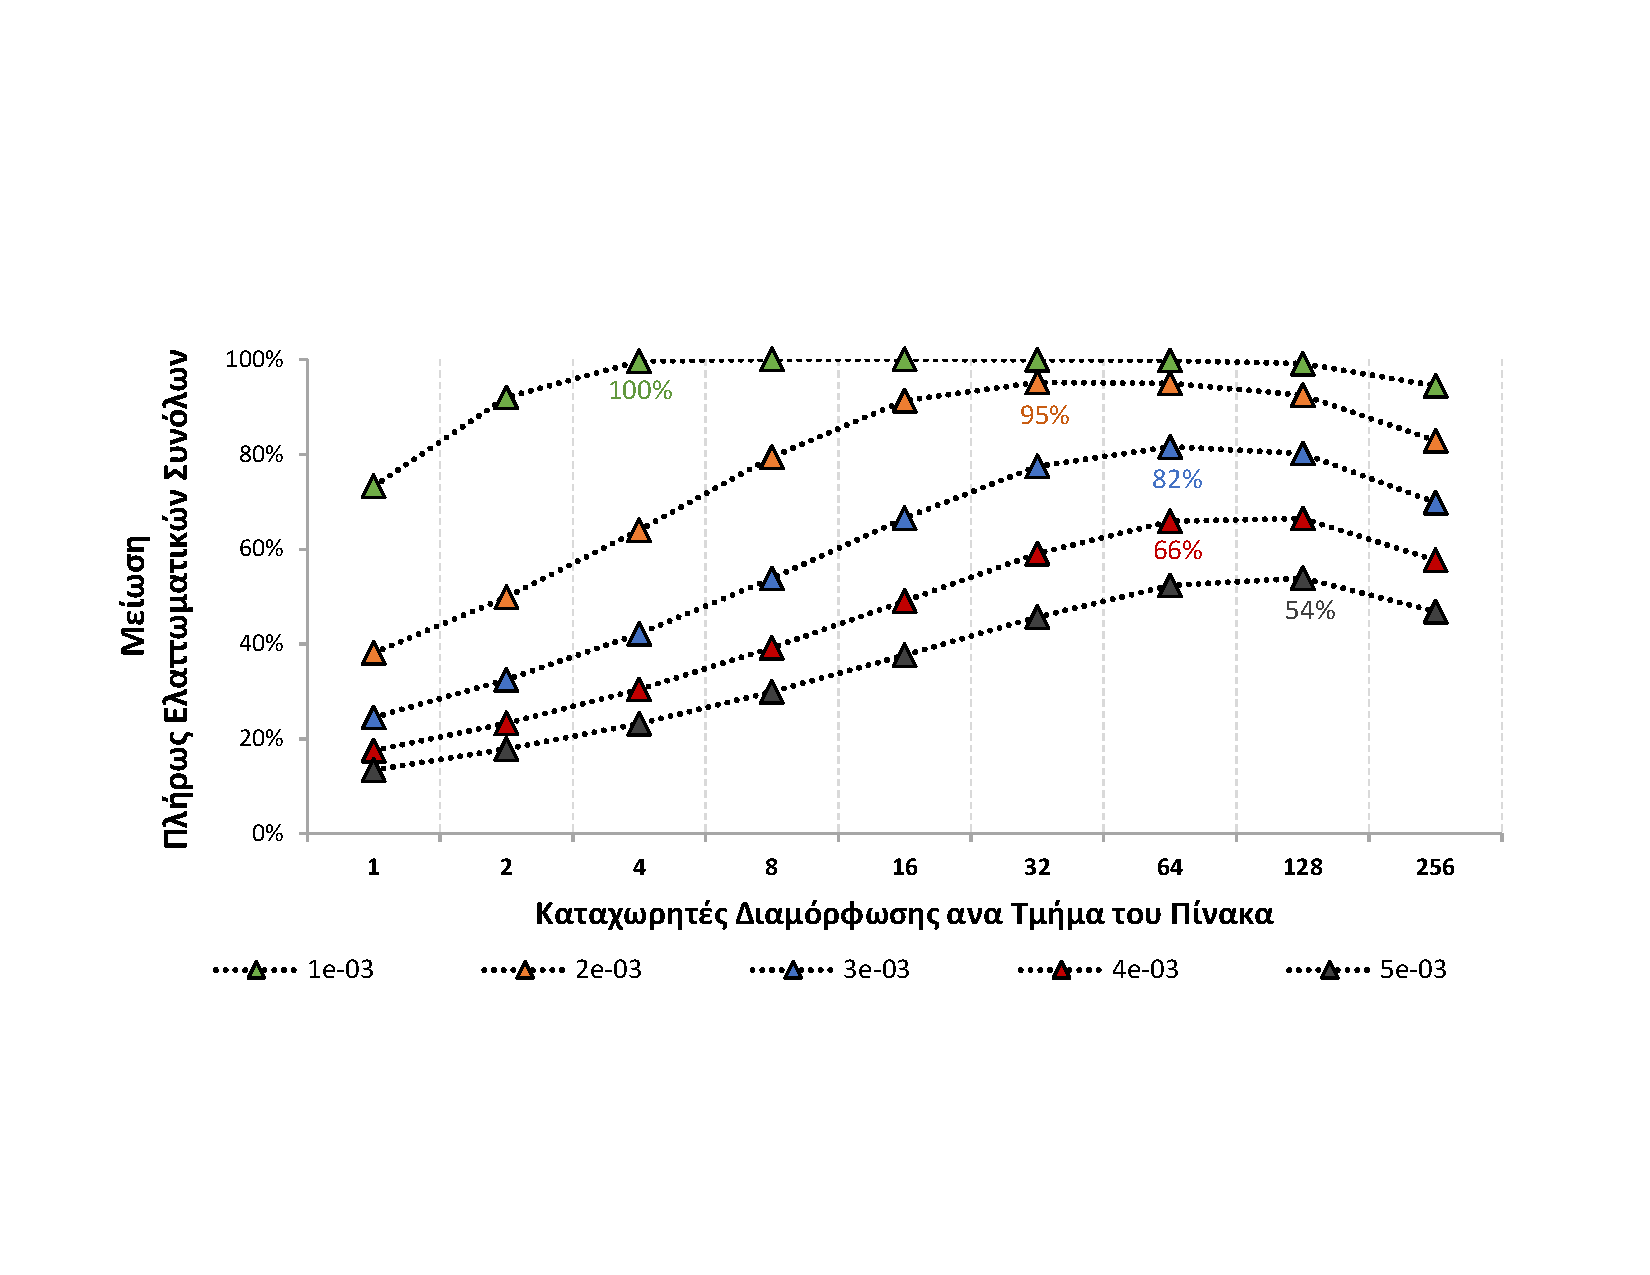
\includegraphics[width=0.99\linewidth, trim=1.9cm 5cm 1.8cm 5.9cm, clip=true]{\resultsDIR/chap5_BTB_ffsets_reduction_2048_2way.pdf}}
        \caption{ΠΠΠΔ 2048-πλαισίων / 2-τρόπων συνόλου συσχέτισης}
        \label{fig:chap5_btb_ffsets_2048_2way}
    \end{subfigure}
    
    \begin{subfigure}[t]{\textwidth}
        \centering
        \fbox{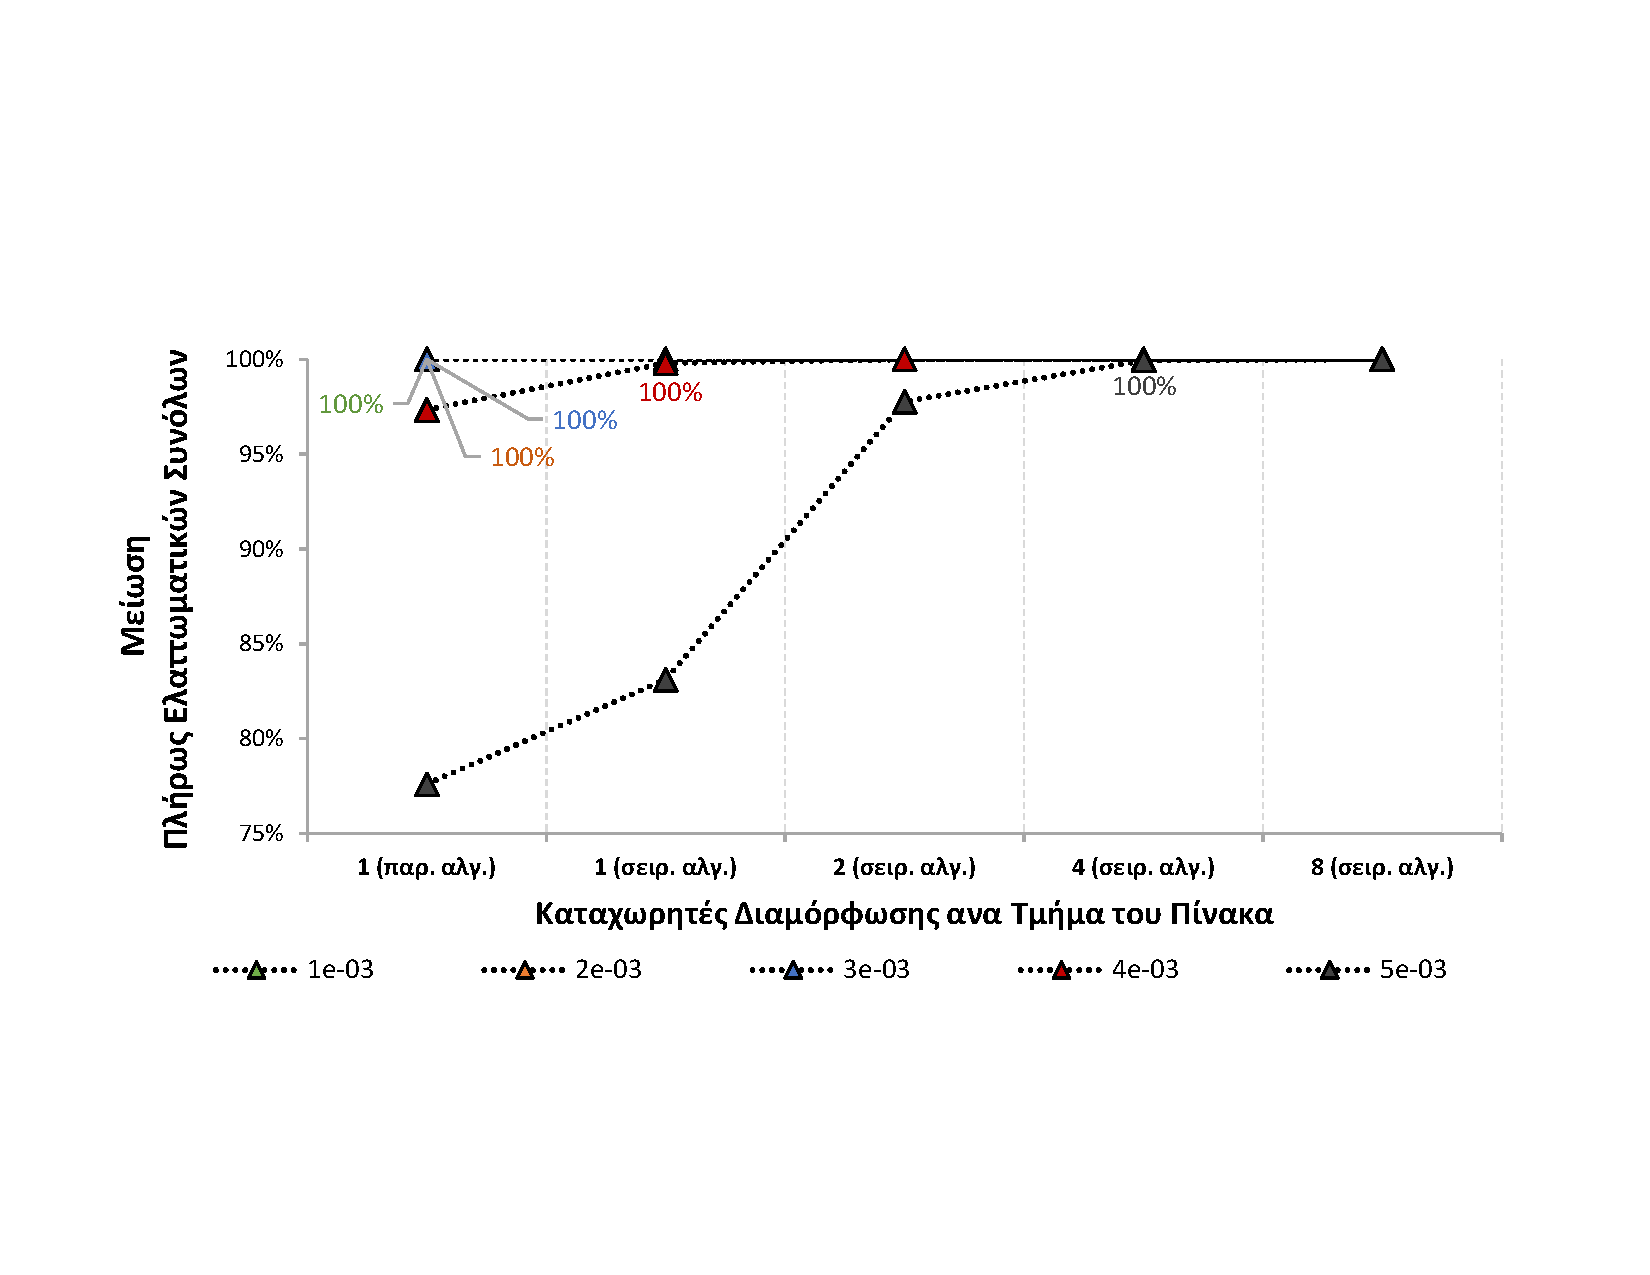
\includegraphics[width=0.99\linewidth, trim=1.9cm 5cm 1.8cm 5.9cm, clip=true]{\resultsDIR/chap5_BTB_ffsets_reduction_2048_4way.pdf}}
        \caption{ΠΠΠΔ 2048-πλαισίων / 4-τρόπων συνόλου συσχέτισης}
        \label{fig:chap5_btb_ffsets_2048_4way}
    \end{subfigure}
    \caption{Μείωση των πλήρως ελαττωματικών πλαισίων με τη χρήση παραλλαγών της μεθόδου, σε σχέση με τη μη εφαρμογή τεχνικής για τη μείωσή τους}
    \label{fig:chap5_btb_ffsets_2048}
\end{figure}

Στο Σχήμα \ref{fig:chap5_btb_ffsets_2048_4way} παρουσιάζονται τα αντίστοιχα αποτελέσματα για τον πίνακα 2048-πλαισίων/4-τρόπων. Ομοίως με το πρώτο γράφημα, κάθε σημείο του οριζόντιου άξονα αντιστοιχεί στη χρήση ενός πλήθους καταχωρητών ανά τμήμα. Συγκεκριμένα, το πρώτο και το δεύτερο σημείο κάθε καμπύλης εκφράζει τα αποτελέσματα της περίπτωσης όπου χρησιμοποιείται ένας καταχωρητής ανά τμήμα και ο υπολογισμός κατάλληλων τιμών γίνεται με τη χρήση του παράλληλου και του σειριακού αλγορίθμου αντίστοιχα.
\par
Όπως φανερώνει και το γράφημα, σε σχετικά μικρές πιθανότητες σφάλματος ($\expnum{1}$, $\expnum{2}$ και $\expnum{3}$) και οι δύο εκδοχές πετυχαίνουν την ολοκληρωτική εξάλειψη των πλήρως ελαττωματικών συνόλων. Αντιθέτων, όταν η πιθανότητα σφάλματος αυξάνεται σε $\expnum{4}$ και $\expnum{5}$ ο σειριακός αλγόριθμος παρουσιάζει αποδοτικότερα αποτελέσματα απ' ότι ο παράλληλος. Συγκεκριμένα, στην πιθανότητα σφάλματος $\expnum{4}$ ο σειριακός αλγόριθμος με χρήση ενός και μόνο καταχωρητή ανά τμήμα είναι σε θέση να εξαλείψει τα πλήρως ελαττωματικά σύνολα, ενώ στην πιθανότητα $\expnum{5}$ πετυχαίνει ποσοστό μείωσης 83\% από 78\% που πετυχαίνει ο παράλληλος. Η διαφορά αυτή οφείλεται στο γεγονός πως τα παράλληλα βήματα του αλγορίθμου εκτελούνται ανεξάρτητα. Για το λόγο αυτό, ο παράλληλος αλγόριθμος αποτελεί πειραματικό αντικείμενο και δεν συνιστάται η χρήση του όταν η μελετώμενη πιθανότητα σφάλματος είναι αυξημένη. Για την ολοκληρωτική εξάλειψης των πλήρως ελαττωματικών συνόλων στην περίπτωση της πιθανότητας σφάλματος $\expnum{4}$ απαιτείται η χρήση τουλάχιστον 4 καταχωρητών ανά τμήμα, όπως φαίνεται και από τους δείκτες γκρι αποχρώσεων του Σχήματος \ref{fig:chap5_btb_ffsets_2048_4way}.
\par
Μία πολύ σημαντική παρατήρηση που εξήχθη από τη μελέτη 1000 χαρτών σφαλμάτων για διαφορετικά μεγέθη του Πίνακα Πρόβλεψης Προορισμού Διακλάδωσης (ΠΠΠΔ) είναι η συσχέτιση του αριθμού Καταχωρητών Διαμόρφωσης που χρησιμοποιούνται με το πλήθος συνόλων που ανήκουν σε κάθε υποτμήματος. Τα γραφήματα του Σχήματος \ref{fig:chap5_btb_ffsets} παρουσιάζουν τη μείωση του αριθμού των πλήρως ελαττωματικών συνόλων σε σχέση με τη μή χρήση κάποια τεχνική, για διαφορετικές διασπάσεις των τμημάτων σε υποτμήματα, δηλαδή διαφορετικά πλήθη συνόλων ανά καταχωρητή διαμόρφωσης. Η μελέτη πραγματοποιήθηκε για μνήμες 512, 1024, 2048 και 4096 πλαισίων.
\par
Στο γράφημα του Σχήματος \ref{fig:chap5_btb_ffsets_2way} που αναφέρεται στην περίπτωση οργάνωσης 2-τρόπων συνόλου συσχέτισης, παρατηρούμε πως για τις πιθανότητες σφάλματος $\expnum{1}$, $\expnum{2}$, $\expnum{3}$, $\expnum{4}$ και $\expnum{5}$ οι κατάλληλες επιλογές συνόλων ανά καταχωρητή είναι 256, 32, 16, 8 και 8 αντίστοιχα. Η μείωση των πλήρως ελαττωματικών συνόλων σε αυτές τις περιπτώσεις θα είναι 100\%, 95\%, 82\%, 67\% και 54\% ανεξαρτήτως μεγέθους. Επομένως, τα βέλτιστα αποτελέσματα που επισημάνθηκαν στην περίπτωση του πίνακα 2048-πλαισίων του Σχήματος \ref{fig:chap5_btb_ffsets_2048_2way} αντιστοιχούν σε αυτές τις βέλτιστες διασπάσεις των συνόλων. Όπως και στην περίπτωση του πίνακα 2048-πλαισίων/2-τρόπων, η μεγάλη διάσπαση των συνόλων μπορεί να επιφέρει αρνητικά αποτελέσματα όπως φαίνεται και από τα τελευταία σημεία των καμπυλών του Σχήματος \ref{fig:chap5_btb_ffsets_2way}.
\par
Το γράφημα του Σχήματος \ref{fig:chap5_btb_ffsets_4way} αναφέρεται στην αντίστοιχη μελέτη μνημών οργάνωσης 4-τρόπων συνόλου συσχέτισης. Αριθμώντας τα σημεία των καμπυλών από αριστερά προς τα δεξιά, τα μονά σημεία αντιστοιχούν στα αποτελέσματα όταν χρησιμοποιείται ο παράλληλος αλγόριθμος για τον υπολογισμό κατάλληλων τιμών, ενώ τα ζυγά στα αποτελέσματα όταν χρησιμοποιείται ο σειριακός. Όπως και στην περίπτωση του πίνακα 2048-πλαισίων του Σχήματος \ref{fig:chap5_btb_ffsets_2048_4way}, στις  πιθανότητες σφάλματος $\expnum{1}$, $\expnum{2}$ και $\expnum{3}$ είναι δυνατή η επίτευξη ολοκληρωτικής εξάλειψης των πλήρως ελαττωματικών συνόλων. Αντιθέτως, όταν οι πιθανότητα σφάλματος αυξάνεται σε $\expnum{4}$ και $\expnum{5}$, για να επιτευχθεί η ολοκληρωτική τους εξάλειψη πρέπει τα σύνολα να διασπαστούν σε τμήματα των 128 συνόλων το κάθε ένα.

\begin{figure}[!t]
    \centering
    \begin{subfigure}[t]{\textwidth}
        \centering
        \fbox{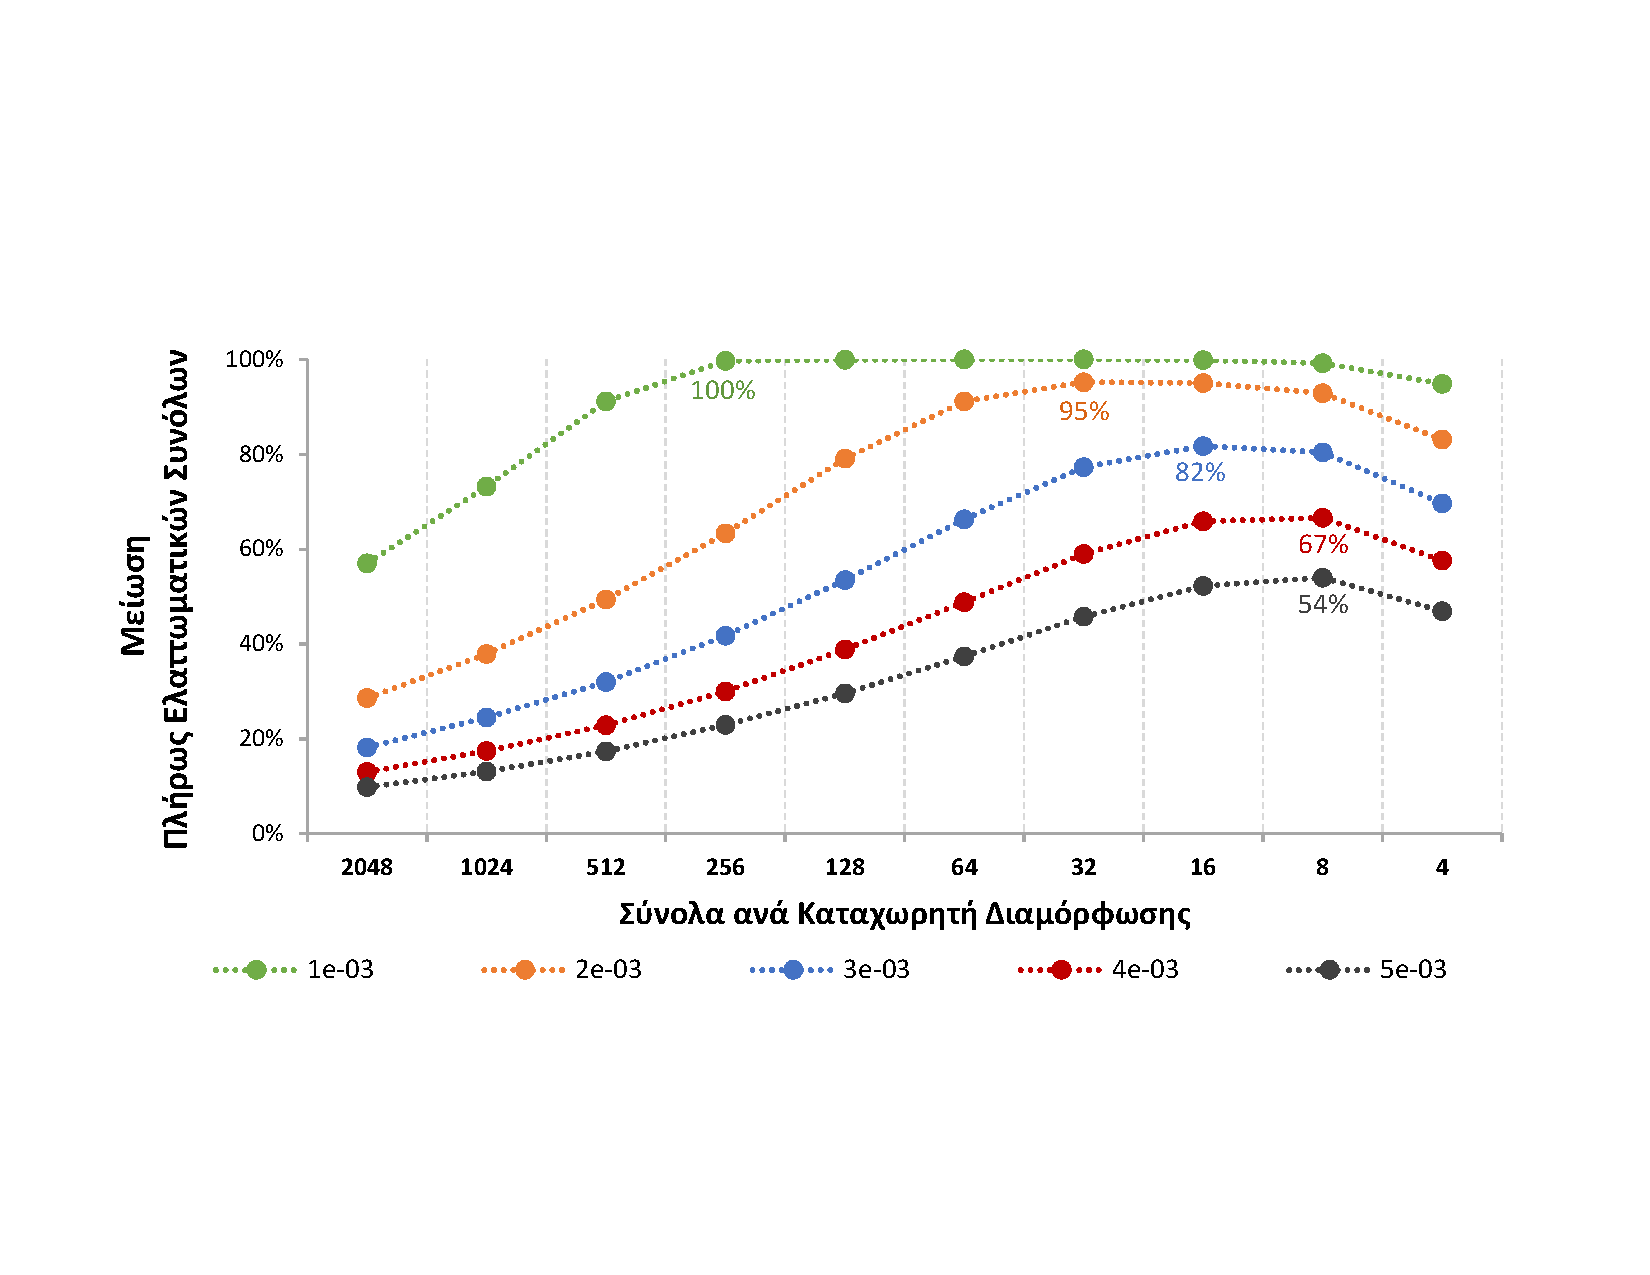
\includegraphics[width=0.99\linewidth, trim=1.9cm 5cm 1.8cm 5.9cm, clip=true]{\resultsDIR/chap5_BTB_ffsets_reduction_2way.pdf}}
        \caption{ΠΠΠΔ 2-τρόπων συνόλου συσχέτισης}
        \label{fig:chap5_btb_ffsets_2way}
    \end{subfigure}
    
    \begin{subfigure}[t]{\textwidth}
        \centering
        \fbox{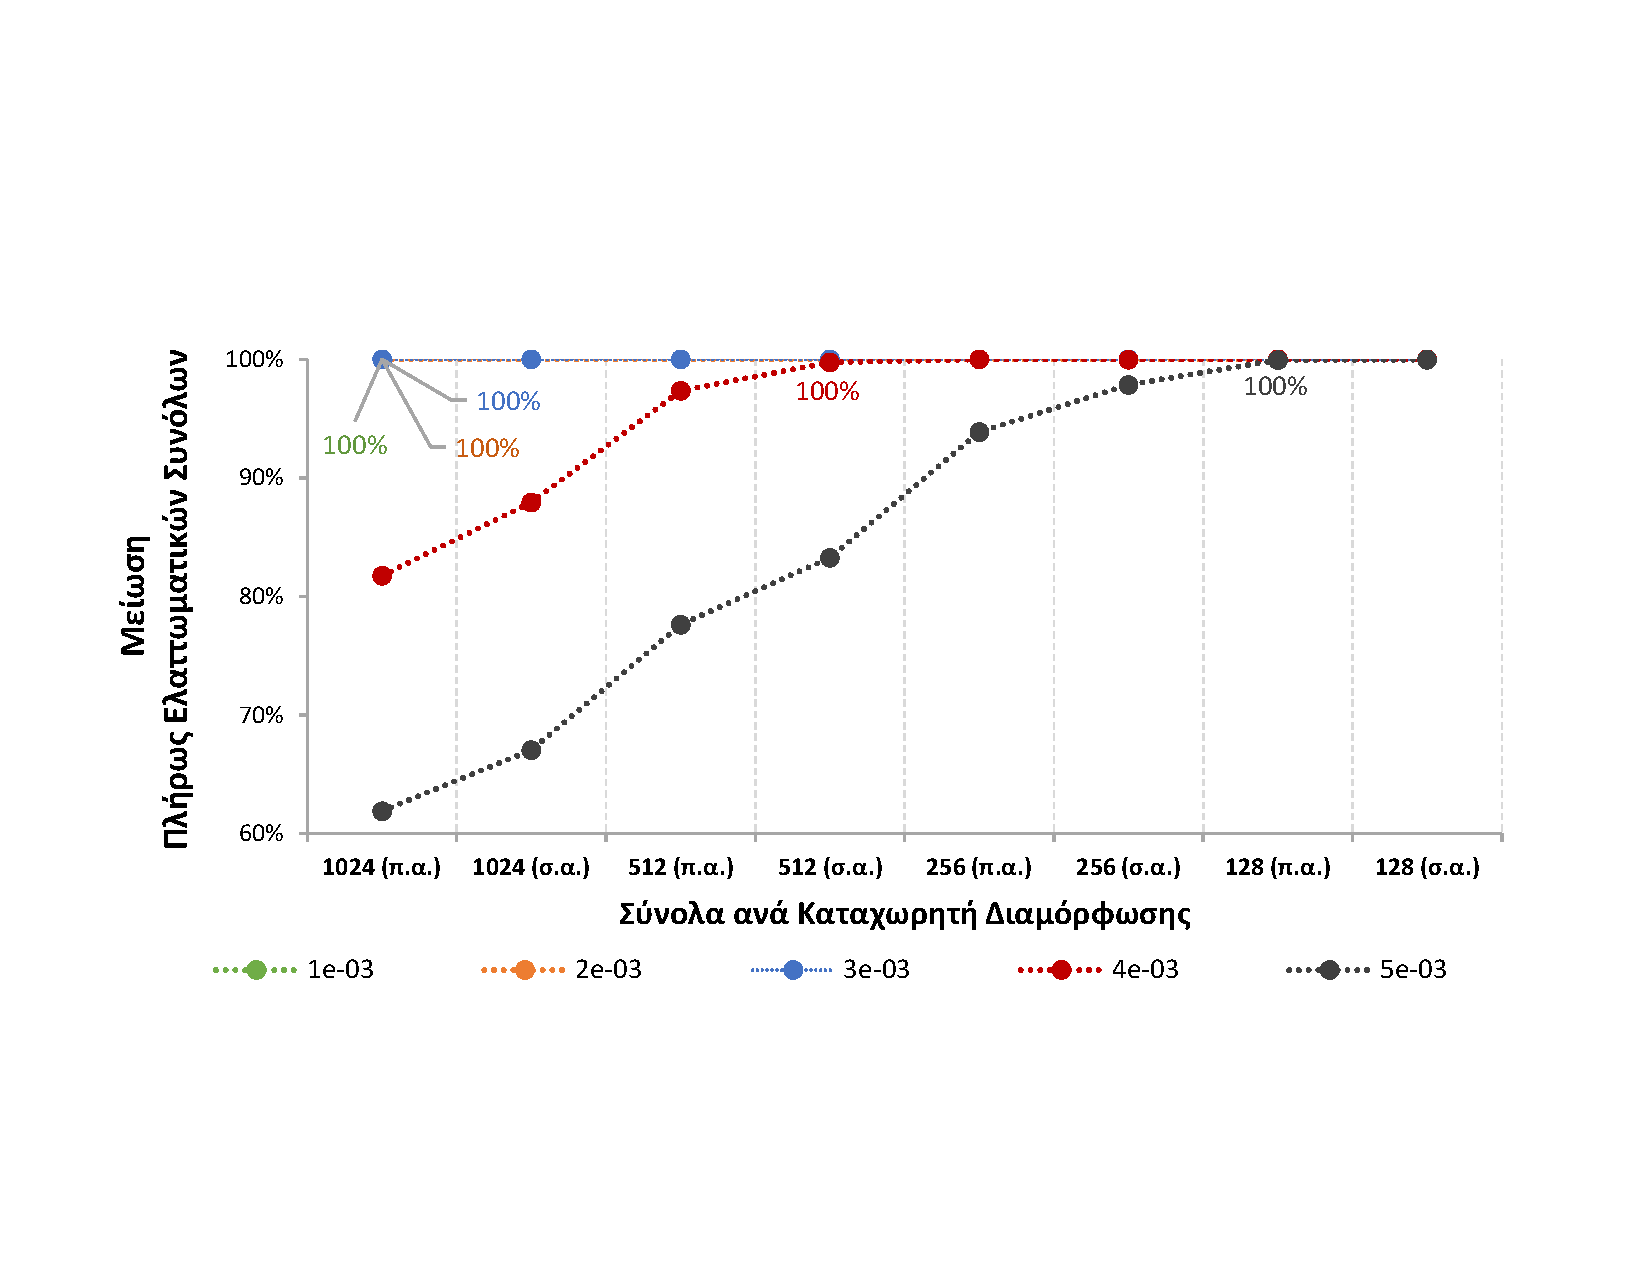
\includegraphics[width=0.99\linewidth, trim=1.9cm 5cm 1.8cm 5.9cm, clip=true]{\resultsDIR/chap5_BTB_ffsets_reduction_4way.pdf}}
        \caption{ΠΠΠΔ 4-τρόπων συνόλου συσχέτισης}
        \label{fig:chap5_btb_ffsets_4way}
    \end{subfigure}
    \caption{Μείωση των πλήρως ελαττωματικών πλαισίων με τη χρήση παραλλαγών της μεθόδου σε σχέση με τη μη εφαρμογή τους}
    \label{fig:chap5_btb_ffsets}
\end{figure}

%----------------------------------------------------------%

\section{Προσέγγιση Χειρότερης Περίπτωσης}
\label{chap5_maxFFSets_num}

Μελετώντας προσεκτικά τον αλγόριθμο εξάγεται ένα πολύ σημαντικό συμπέρασμα, η δυνατότητα εύρεσης του μέγιστου αριθμού πλήρως ελαττωματικών συνόλων που μπορεί να προκύψουν μετά την εφαρμογή της τεχνικής. Η μόνη γνώση που απαιτείται είναι το πλήθος ελαττωματικών πλαισίων ανά τμήμα. Το δεδομένο αυτό αποτελεί μία εκτίμηση του αποτελέσματος του αλγορίθμου, για την χειρότερη περίπτωση κατανομής των ελαττωματικών πλαισίων.
\par
Έστω ότι $f_1$ και $f_2$ το πλήθος των σφαλμάτων στα δύο τμήματα ενός Πίνακας Πρόβλεψης Προορισμού Διακλάδωσης 2-τρόπων, με $S$ σύνολα συσχέτισης. Στην χειρότερη περίπτωση αρχικής κατανομής των σφαλμάτων, η εφαρμογής της πρώτης μεθόδου θα περιόριζε τα πλήρως ελαττωματικά σύνολα σε:

\begin{equation}
    \label{eqn:chap5_maxFFSETS_2way}
    X = \floor*{ \frac{f_1 \times f_2}{S} }
\end{equation}

Η εξίσωση αυτή προέρχεται από το γεγονός ότι οι πράξεις \xor που πραγματοποιούνται μεταξύ των δύο τμημάτων, θα είναι όσο και το γινόμενο του πλήθους ελαττωματικών πλαισίων τους ($f_1 \times f_2$), όπως αναφέρθηκε και στην ανάλυση των παραδειγμάτων. Η σχέση \ref{eqn:chap5_maxFFSETS_2way} μπορεί να γίνει κατανοητή από ένα παράδειγμα όπου για κάθε εκτέλεση μίας πράξης \xor ενημερώνεται διαφορετικός μετρητής, ώστε οι μετρητές να αυξάνονται ομοιόμορφα τελικά (για παράδειγμα: $XFB=000 \rightarrow XFB=001 \rightarrow XFB=010 \rightarrow ... \rightarrow XFB=111 \rightarrow XFB=000 \rightarrow XFB=001 \rightarrow ... $). Συνεπώς, εάν όλα τα πλαίσια είναι ελαττωματικά τότε κάθε μετρητής θα έχει την τιμή $S$. Στην περίπτωσης ομοιόμορφης αύξησης η επιλογή κατάλληλης τιμής γίνεται δυσκολότερη, σε αντίθεση με την περίπτωση όπου ένα αποτέλεσμα επαναλαμβάνεται περισσότερες φορές, και επομένως ο αντίστοιχος μετρητής-α αυξάνεται περισσότερες φορές σε σχέση με ένα μετρητή-β (το σύνολο των αυξήσεων παραμένει σταθερό). Έτσι η τιμή που αντιστοιχεί στον μετρητή-β είναι η επιθυμητή.
\par
Μέσω της εξίσωσης \ref{eqn:chap5_maxFFSETS_2way} μπορεί να γίνει μία εκτίμηση της χειρότερης περίπτωσης προτού γίνει η εκτέλεση του αλγορίθμου. Η στρογγυλοποίηση του αριθμού προς τον πλησιέστερο μικρότερο ακέραιο αριθμό (\en{floor}) γίνεται διότι το πλήθος των πλήρως ελαττωματικών συνόλων είναι ακέραιος αριθμός.
\par
Για την περίπτωση ενός Πίνακας Πρόβλεψης Προορισμού Διακλάδωσης 4-τρόπων με πλήθος σφαλμάτων ανά τμήμα $f_1, f_2, f_3$ και $f_4$ αντίστοιχα, το όριο αυτό υπολογίζεται ως:

\begin{equation}
    \label{eqn:chap5_maxFFSETS_X}
    X = \floor*{ \frac{ \floor*{ \frac{ \floor*{ \frac{f_1 \times f_2}{S} } \times f_3}{S} } \times f_4}{S} }
\end{equation}

\noindent όπου $f_i$ είναι το πλήθος ελαττωματικών πλαισίων του Τμήματος-$i$ και $S$ ο αριθμός συνόλων του Πίνακας Πρόβλεψης Προορισμού Διακλάδωση, όπως προαναφέρθηκε.
\par
Η σχέση \ref{eqn:chap5_maxFFSETS_X} συνεπάγεται από το ότι ο αλγόριθμος εκτελείται σειριακά και για κάθε βήμα του χρησιμοποιούνται οι άλυτες περιπτώσεις του προηγούμενου βήματος. Επομένως, για τον υπολογισμό της χειρότερης περίπτωσης, αρκεί να γίνει η υπόθεση πως σε κάθε βήμα χρησιμοποιείται η χειρότερη περίπτωση αποτελέσματος του προηγούμενου βήματος.

%----------------------------------------------------------%

\section{Υλοποίηση της Τεχνικής στο Υλικό}
\label{chap5_HardwareImplementation}

Η υλοποίηση της τεχνικής απαιτεί ελάχιστη αύξηση του υλικού. Για παράδειγμα σε ένα πίνακα 2048-πλαισίων/2-τρόπων στον οποίο χρησιμοποιούνται 64 καταχωρητές ανά τμήμα, τα στοιχεία που απαιτούνται είναι 128 καταχωρητές των 4 δυαδικών ψηφίων για την αποθήκευση πληροφορίας (512 κυψελίδες συνολικά), καθώς και 512 πύλες \xor ενός επιπέδου. Επομένως, η αύξηση θα είναι μικρότερη από 1\% . Αυτό αποτελεί πολύ σημαντικό γεγονός εάν συγκριθεί η συγκεκριμένη τεχνική με ήδη υπάρχουσες τεχνικές για Κρυφές Μνήμες Δεδομένων και Εντολών, όπως για παράδειγμα η \cite{shirvani1999padded} με την οποία θα ήταν δυνατή η πλήρης εξάλειψη των πλήρως ελαττωματικών συνόλων μέσω της ανακατεύθυνσης των ελαττωματικών πλαισίων σε υγιή, όμως με μία αύξηση του υλικού μεγαλύτερη του 20\%.
\par
Στα Σχήματα \ref{fig:chap5_permutation_impl_v1} και \ref{fig:chap5_permutation_impl_v2} όπου αναδεικνύεται η υλοποίηση της τεχνικής, παρουσιάζονται δύο διαφορετικές εκδοχές, ώστε να αφήνεται στο σχεδιαστή η απόφαση του τρόπου υλοποίησης αναλόγως του κόστους κάθε μίας. Η πρώτη υλοποίηση απαιτεί τη χρησιμοποίηση πολλαπλών μικρότερων αποκωδικοποιητών, το οποίο μπορεί να επιφέρει μικρή αύξηση στην κατανάλωση και την επιφάνεια. Η δεύτερη υλοποίηση απαιτεί την προσθήκη πολυπλεκτών στο μονοπάτι της διευθυνσιοδότηση ώστε να επιλέγεται ο κατάλληλος Καταχωρητής Διαμόρφωσης. Η λύση αυτή μπορεί να επιφέρει αύξηση της απαιτούμενης επιφάνειας και πιθανώς μικρή καθυστέρηση στην εξαγωγή δεδομένου από τον Πίνακα Πρόβλεψης Προορισμού Διακλάδωσης. Τέλος, θα μπορούσε να γίνει ενσωμάτωση μίας υβριδικής υλοποίησης όπου χρησιμοποιούνται λιγότεροι πολυπλέκτες σε συνδυασμό με ένα μικρό πλήθος αποκωδικοποιητών. Το κόστος για κάθε υλοποίηση εξαρτάται άμεσα από την τεχνολογία που χρησιμοποιεί κάθε σχεδιαστής.

\begin{figure}[h]
    \centering
    \fbox{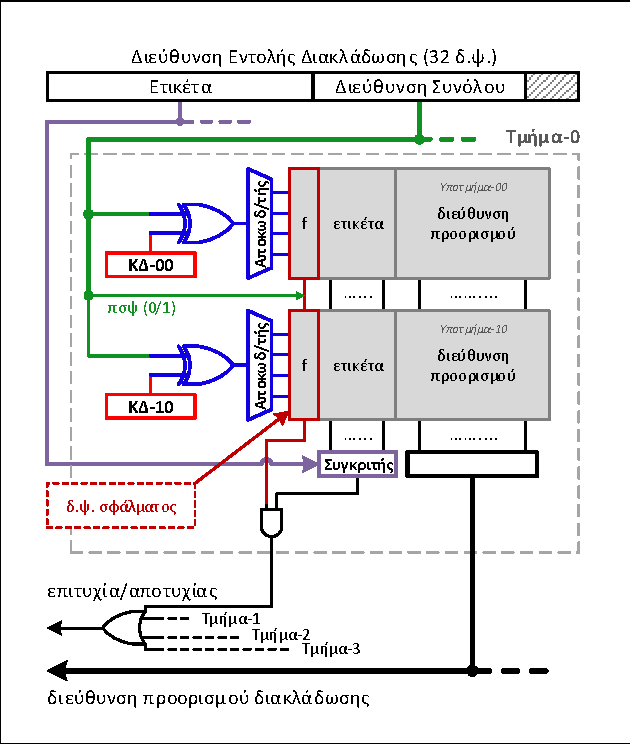
\includegraphics[width=0.8\linewidth,trim=0.5cm 0.6cm 0.5cm 0.8cm, clip=true]{\hardwareDIR/chap5_high_level_diagram_v1.pdf}}
    \caption{1\textsuperscript{ος} Τρόπος Υλοποίησης - Διάσπαση αποκωδικοποιητή}
    \label{fig:chap5_permutation_impl_v1}
\end{figure}

\begin{figure}[t]
    \centering
    \fbox{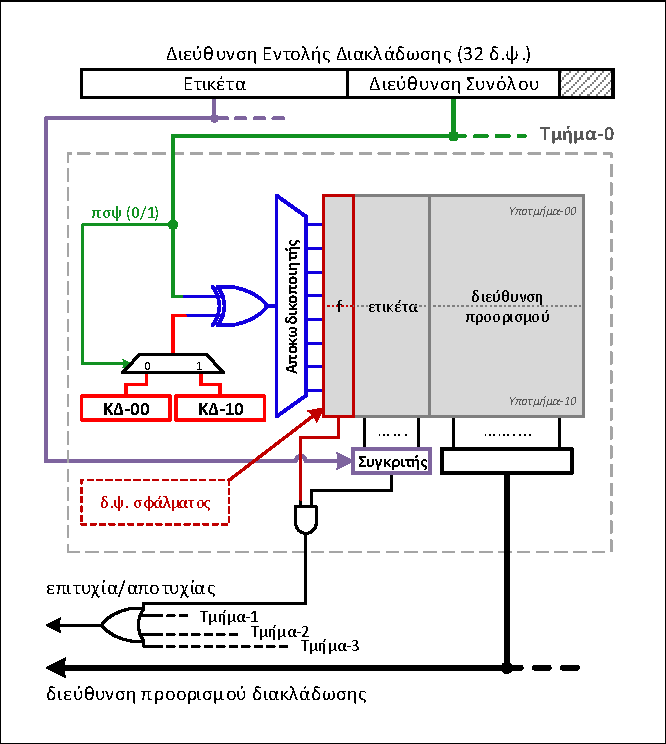
\includegraphics[width=0.8\linewidth,trim=0.5cm 0.6cm 0.5cm 0.6cm, clip=true]{\hardwareDIR/chap5_high_level_diagram_v2.pdf}}
    \caption{2\textsuperscript{ος} Τρόπος Υλοποίησης - Προσθήκη πολυπλέκτη}
    \label{fig:chap5_permutation_impl_v2}
\end{figure}

Παρά το γεγονός πως η διάσπαση σε υποτμήματα συνεπάγεται και μερική αύξηση της κατανάλωσης του Πίνακα Πρόβλεψης Προορισμού Διακλάδωσης, η μείωση του χρόνου ολοκλήρωσης ενός προγράμματος εξαιτίας της μεγάλης μείωσης των πλήρως ελαττωματικών συνόλων θα οδηγήσει τελικώς σε σημαντική μείωση της συνολικής κατανάλωσης του ολοκληρωμένου κυκλώματος. Τα αποτελέσματα τόσο της μείωσης της κατανάλωσης όσο και της απώλειας που υφίσταται η απόδοση του υπερβαθμωτού επεξεργαστή παρουσιάζονται στο Κεφάλαιο \ref{chap6}.


%----------------------------------------------------------%
